\documentclass[a4paper,11pt]{report}
%\usepackage[none]{hyphenat}

%\usepackage[T1]{fontenc}
%\usepackage[bitstream-charter]{mathdesign}

%\usepackage[usenames,dvipsnames,pdf]{pstricks}
%\usepackage[crop=off]{auto-pst-pdf}
\usepackage{makeidx}
\usepackage{url}
\usepackage[square,sort,comma,numbers]{natbib}
\usepackage{framed}
\usepackage{svg}
\usepackage{graphicx}
\usepackage{longtable}
\usepackage{amsfonts}
\usepackage{amsmath}
\usepackage{float}

\usepackage[noend,ruled,noline,linesnumbered,algochapter]{algorithm2e}

% --- TikZ, for the agentic-loop and pipeline diagrams (Chapters 3 and 4) ------
\usepackage{tikz}
\usetikzlibrary{arrows.meta, positioning, shapes.geometric, calc, fit,
                backgrounds, decorations.pathreplacing}
\usepackage{xcolor}

% ── Prompt listings ───────────────────────────────────────────────────────
% The CoT and PoT prompts are reproduced verbatim in Chapter 3, and the prompt
% IS the method there, so they are set as framed, captioned, cross-referenceable
% listings rather than as loose verbatim blocks. breaklines lets a long prompt
% line wrap on its own instead of being hand-wrapped to fit the column, which
% would misrepresent the prompt's real line structure.
\usepackage{listings}
\definecolor{promptbg}{HTML}{F7F8FA}
\definecolor{promptrule}{HTML}{C3C8D2}
\definecolor{promptkey}{HTML}{0B4F6C}
\lstdefinestyle{prompt}{
  basicstyle=\ttfamily\small,
  backgroundcolor=\color{promptbg},
  frame=single,
  rulecolor=\color{promptrule},
  framesep=6pt,
  xleftmargin=10pt,
  xrightmargin=10pt,
  % Hyphen counts as a word character, otherwise listings tokenises
  % CHAIN-OF-THOUGHT into CHAIN / OF / THOUGHT and the emph never matches.
  alsoletter={-},
  breaklines=true,
  breakatwhitespace=false,
  breakindent=14pt,
  postbreak=\mbox{\textcolor{promptrule}{$\hookrightarrow$}\space},
  columns=fullflexible,
  keepspaces=true,
  showstringspaces=false,
  captionpos=b,
  abovecaptionskip=6pt,
  emph={CHAIN-OF-THOUGHT,PROGRAM-OF-THOUGHT,STRICT,MUST,EACH,EQUALS,BEFORE},
  emphstyle=\bfseries\color{promptkey},
}
\renewcommand{\lstlistingname}{Prompt}

% LectureAssist palette -- kept identical to the project poster so that the
% report and the poster read as one visual system.
\definecolor{LAindigo}{HTML}{6366F1}
\definecolor{LAviolet}{HTML}{A78BFA}
\definecolor{LAcyan}{HTML}{38BDF8}
\definecolor{LAgreen}{HTML}{34D399}
\definecolor{LAamber}{HTML}{FBBF24}
\definecolor{LAred}{HTML}{F87171}
\definecolor{LAink}{HTML}{2B2C45}
\definecolor{LAmist}{HTML}{EEF0FD}
\definecolor{LAslate}{HTML}{64748B}

\tikzset{
  labox/.style={rectangle, rounded corners=3pt, draw=LAindigo, line width=0.9pt,
    fill=white, text=LAink, align=center, inner sep=4pt, minimum height=9mm,
    font=\small\bfseries},
  laproc/.style={labox, draw=LAviolet, fill=LAviolet!8},
  lallm/.style={labox, draw=LAamber, fill=LAamber!15},
  laout/.style={labox, draw=LAgreen, fill=LAgreen!12},
  laval/.style={labox, draw=LAred, fill=LAred!8},
  latool/.style={labox, draw=LAcyan, fill=LAcyan!10, dashed},
  laarr/.style={-{Stealth[length=2.4mm,width=1.8mm]}, line width=0.9pt,
    draw=LAindigo},
  laarrg/.style={-{Stealth[length=2.4mm,width=1.8mm]}, line width=0.9pt,
    draw=LAgreen},
  laloop/.style={-{Stealth[length=2.4mm,width=1.8mm]}, line width=0.9pt,
    draw=LAred},
  laarrc/.style={-{Stealth[length=2.4mm,width=1.8mm]}, line width=0.8pt,
    draw=LAcyan, dashed},
  lalbl/.style={font=\scriptsize\itshape, text=LAink, fill=white, inner sep=1.5pt},
}


\usepackage[linktoc=page]{hyperref}
\usepackage[margin=3cm]{geometry}
\usepackage{setspace} 


\usepackage{fancyhdr}
\pagestyle{fancy}
\fancyhf{} % clear all headers and footers
\fancyhead[R]{\nouppercase{\leftmark}} % chapter title only
\fancyfoot[C]{\thepage}
\setlength{\headheight}{15pt}
\setlength{\headsep}{12pt}

% \rhead{\nouppercase\leftmark}
% \lhead{\nouppercase\rightmark}

\makeindex

\onehalfspacing 

\renewcommand*\contentsname{Table of Contents}

\begin{document}

\pagenumbering{roman}

%hardbound cover page (foil-stamped); must come before the inner title page
% ============================================================================
%  Hardbound cover page.
%
%  This is the page that is foil-stamped on the bound copy, so it sits BEFORE
%  the inner title page (0.0.title.tex) and deliberately carries no page number
%  and no running head.
%
%  It differs from the inner title page in two ways on purpose: the date is
%  fixed ("August 2026") rather than \today, because a bound cover must not
%  change every time the document is recompiled, and the supervisor is named
%  with his rank as it should appear on the binding.
%
%  \singlespacing is set locally because the document runs \onehalfspacing;
%  without it the block is about 1.5cm too tall and the closing department
%  lines spill onto a second page.
% ============================================================================
\begin{titlepage}
\thispagestyle{empty}
\begin{singlespace}

\begin{center}

\vspace*{0.8cm}

{\LARGE \bf LectureAssist:}\\[0.6em]
{\Large \bf An Agentic, Multimodal AI Assistant}\\[0.35em]
{\Large \bf that Turns Lectures into Adaptive Study Material}

\vspace{1.2cm}

{\large By}

\vspace{0.7cm}

{\large \bf Iftikhar Ahmed \quad 2121019642}\\[0.35em]
{\large \bf Salman Shafi \quad 2211386042}\\[0.35em]
{\large \bf Jarinah Tasnim \quad 2121026642}

\vspace{1.8cm}

Submitted in partial fulfillment of the requirements\\
of the degree of Bachelor of Science in Computer Science and Engineering

\vspace{1.0cm}

{\large August 2026}

\vspace{0.8cm}


\includegraphics[scale=0.15]{./NSU}

\vspace{0.7cm}

{\large Department of Electrical and Computer Engineering}\\[0.3em]
{\large North South University}

\end{center}

\end{singlespace}
\end{titlepage}


%title page
\begin{titlepage}


\begin{center}
\line(1,0){430}\\
%{ \Huge \bf Heuristically Guided\\ Local Search for \\ Protein Structure Prediction \\}
{\Huge \bf LectureAssist:\\ \vspace{.5em} An Agentic, Multimodal AI Assistant that\\ \vspace{.3em} Turns Lectures into Adaptive Study Material}
\line(1,0){430}

\end{center}

\vfill

\begin{center}
By
\end{center}

\vfill
\begin{center}
{\large \bf Iftikhar Ahmed --- ID \# 2121019642}\\
{\large \bf Salman Shafi --- ID \# 2211386042}\\
{\large \bf Jarinah Tasnim --- ID \# 2121026642}\\
\end{center}

\vfill

\begin{center}
{\large Supervised by}\\
\vspace{.4em}
{\large \bf Dr. Adnan Areefen}\\
{Department of Electrical and Computer Engineering}\\
{North South University}
\end{center}


\vfill


\begin{center}
{Submitted in partial fulfillment of the requirements \\of the degree of Bachelor of Science in Computer Science and Engineering}
\end{center}

\vfill
\begin{center}
{\today}
\end{center}

\vfill
	
\begin{center}

\includegraphics[scale=0.15]{./NSU}
\end{center}

\begin{center}
	\textsc{Department of Electrical and Computer Engineering\\
		North South University}
\end{center}



\end{titlepage}



%\clearpage
%\thispagestyle{empty}
%\mbox{}
\clearpage

%\thispagestyle{empty}
%Dedication
%I would like to dedicate this thesis to my loving family ...
    



%\clearpage
%\thispagestyle{empty}
%\mbox{}
%\clearpage
%\thispagestyle{empty}
\pagenumbering{roman}
\setcounter{page}{1}


\begin{titlepage}

\begin{center}
\line(1,0){430}\\
{\Huge \bf APPROVAL}
\line(1,0){430}
\end{center}

\vfill

\begin{center}
Iftikhar Ahmed (ID \# XXXXXXXXX), Salman Shafi (ID \# XXXXXXXXX), and Jarinah Tasnim (ID \# XXXXXXXXX) \\
from the Department of Electrical and Computer Engineering, North South University \\
have worked on the Senior Design Project titled: \\

\vspace{1em}

{\Large \bf “LectureAssist: An Agentic, Multimodal AI Assistant that Turns Lectures into Adaptive Study Material”}

\vspace{1em}

under the supervision of \textbf{Dr. Adnan Areefen} in partial fulfillment of the requirement \\
for the degree of Bachelor of Science in Computer Science and Engineering and has been accepted as satisfactory.
\end{center}

\vfill
\vfill

% Supervisor Signature Block
\begin{flushleft}
\textbf{Supervisor’s Signature}

\vspace{2em}

…………………………………….

\textbf{Dr. Adnan Areefen} \\
Department of Electrical and Computer Engineering \\
North South University \\
Dhaka, Bangladesh.
\end{flushleft}

\vfill

% Chairman Signature Block
\begin{flushleft}
\textbf{Chairman’s Signature}

\vspace{2em}

…………………………………….

\textbf{Dr. XXX} \\
Professor \\
Department of Electrical and Computer Engineering \\
North South University \\
Dhaka, Bangladesh.
\end{flushleft}

\vfill

\end{titlepage}


\begin{titlepage}

\begin{center}
\line(1,0){430}\\
{\Huge \bf DECLARATION}
\line(1,0){430}
\end{center}

\vfill

\begin{center}
It is to declare that this project is our original work. No part of this work has been
submitted elsewhere, partially or entirely, for the award of any other degree or diploma.
All project related information will remain confidential and shall not be disclosed
without the formal consent of the project supervisor.

\vspace{1em}

Relevant previous works presented in this report have been adequately acknowledged
and cited. The plagiarism policy, as stated by the supervisor, has been maintained.
\end{center}

\vfill
\vfill

\begin{flushleft}
\textbf{Students’ Names \& Signatures}
\end{flushleft}

\vspace{1.5em}

\begin{flushleft}
1. \textbf{Iftikhar Ahmed}

\vspace{1em}
\noindent\_ \_ \_ \_ \_ \_ \_ \_ \_ \_ \_ \_ \_ \_ \_ \_ \_ \_ \_ \_

\vspace{2em}

2. \textbf{Salman Shafi}

\vspace{1em}
\noindent\_ \_ \_ \_ \_ \_ \_ \_ \_ \_ \_ \_ \_ \_ \_ \_ \_ \_ \_ \_

\vspace{2em}

3. \textbf{Jarinah Tasnim}

\vspace{1em}
\noindent\_ \_ \_ \_ \_ \_ \_ \_ \_ \_ \_ \_ \_ \_ \_ \_ \_ \_ \_ \_
\end{flushleft}

\vfill

\end{titlepage}


\clearpage
\begin{center}
{\huge \bf Acknowledgements}
\line(1,0){430}
\end{center}



This work would not have been possible without the input and support of many people
over the last two trimesters. We would like to express our gratitude to everyone who
contributed to it in some way or other.

First and foremost, we would like to thank our supervisor, \textbf{Dr. Adnan Areefen},
Department of Electrical and Computer Engineering, North South University, for his
guidance throughout this project. His insistence that the evaluation be made rigorous
that the generation prompts be shown rather than described, that chain-of-thought
and program-of-thought baselines be compared directly against our agentic pipeline,
and that question generation and answer generation be treated as two separate agents
whose answers must be cross-checked fundamentally shaped this work, and turned it
from a demonstration into a study.

Our sincere gratitude goes to the Department of Electrical and Computer Engineering,
North South University, for providing the academic environment and the resources that
made this project possible.

We are also thankful to the open-source community, whose freely available models and
tools --- Gemma~3, Ollama, Whisper, EasyOCR, Sentence-Transformers and FAISS --- are
the foundation on which this system is built, and without which a project of this
scope could not have been undertaken without significant funding.

Last but not the least, we owe a great deal to our families, including our parents,
for their unconditional love and immense emotional support.


\clearpage
%Abstract
\setlength{\headheight}{14pt}
\begin{center}
	{\huge \bf Abstract}
	\line(1,0){430}
\end{center}

Recorded lectures and digital course material are now abundant, but the tools
that help students convert that material into practice and self assessment are
not. Existing study aids either require the student to paste in clean text by
hand, or depend on paid cloud APIs that are impractical in bandwidth limited and
cost-sensitive settings. This report presents \textbf{LectureAssist}, an
end-to-end agentic AI system that turns a raw lecture video or an academic
document into structured study and assessment material without any proprietary
cloud service. The system couples a dual-channel extraction layer scene-adaptive
optical character recognition that distinguishes slides, blackboards, whiteboards
and on-screen text, combined with Whisper-based speech transcription to a
multi-agent generation pipeline that plans, retrieves, generates, validates and
refines five types of quiz questions, all served by locally hosted Gemma~3 models
through the Ollama runtime on a single consumer-grade GPU. A retrieval augmented
chat interface and an adaptive difficulty engine that tracks per topic performance
complete the loop from raw media to personalised assessment. The system was
evaluated on a large scale study in which multiple-choice questions were generated
from a college-level calculus chapter across three difficulty levels, and scored by
an independent, larger judge model on question quality, grounding, diversity and
separately --- \emph{answer correctness}, using a second Answer Generator agent
that re-solves each question without seeing the marked option. The work demonstrates that high quality, personalised educational AI
is achievable on accessible hardware, and that question generators must be judged
on answer correctness and diversity, not on fluency alone.
\clearpage
\setlength{\headheight}{12pt}




%\input{0.3.pub.tex}






\clearpage
\phantomsection
\tableofcontents
\renewcommand{\contentsname}{Table of Contents}
\addcontentsline{toc}{chapter}{Table of Contents}

\clearpage
\phantomsection
\addcontentsline{toc}{chapter}{List of Figures}
\listoffigures

\clearpage
\phantomsection
\addcontentsline{toc}{chapter}{List of Tables}
\listoftables



\clearpage
\pagenumbering{arabic}
\setcounter{page}{1}

\renewcommand\bibname{References}

\clearpage
\phantomsection


\chapter{Introduction}
\label{ch:intro}

This chapter motivates the project, states its purpose and contributions, and
outlines the structure of the remainder of the report.

\section{Background and Motivation}
\label{sec:intro-motivation}

The proliferation of recorded lectures and digital course material has created a
fundamental imbalance in self directed learning: students have more content than
ever, but fewer tools with which to extract, consolidate and assess their
understanding of it. A single semester course now routinely produces dozens of
hours of recorded lectures, slide decks and reference chapters. Reviewing that
material passively  re-watching a video, re-reading a chapter is one of the
least effective study strategies available. Decades of work in the learning
sciences instead point to \emph{retrieval practice}: repeatedly testing oneself on
the material produces substantially more durable learning than re-exposure to it.
The obstacle is supply. Producing good practice questions is slow, expert work,
and the questions that do exist are concentrated at the end of textbook chapters,
are not tied to what a particular instructor actually emphasised in class, and run
out long before a student has mastered a weak topic.

Existing AI assisted study tools address this gap only partially. Text based
chatbots require the student to manually transcribe or paste lecture content before
they can help, which puts the burden of the hardest step getting the lecture out
of the video and into text back on the student. Cloud dependent question
generation services remove that burden, but they are inaccessible in
bandwidth limited regions, they charge per token at a scale that makes routine
practice expensive, and they require sending course material  which may be
copyrighted or institutionally restricted  to a third party server. Crucially,
none of these tools close the full loop from raw instructional media, through
intelligent content understanding, to graded and personalised assessment without
human intervention at each stage.

There is also a quality problem that is easy to overlook. A large language model
asked to write a multiple choice question will almost always produce something
that \emph{reads} like a good question. Whether the option it marks as correct
actually \emph{is} correct is a separate matter, and one that fluency based
evaluation cannot detect. A study tool that confidently teaches a student the wrong
answer is worse than no tool at all. Any serious system for automatic question
generation therefore has to be evaluated on answer correctness, and on whether it
keeps producing genuinely different questions rather than paraphrasing the same one,
not merely on whether its output is well written.

\section{Purpose and Goal of the Project}
\label{sec:intro-purpose}

The goal of this project is to build and rigorously evaluate \textbf{LectureAssist},
a fully local, API free system that ingests a lecture video or an academic document
and autonomously produces validated, difficulty controlled assessment material,
together with a retrieval grounded chat interface over the same content.

The system is built around three ideas working in concert. First, a
\emph{dualchannel extraction} layer simultaneously processes the visual channel of
a lecture  using scene type adaptive OCR that distinguishes slides, blackboards,
whiteboards and on-screen text, each of which needs different image preprocessing
and its audio channel via Faster Whisper transcription, producing a unified,
timestamped lecture timeline. Second, a \emph{multi-agent generation pipeline}
decomposes quiz creation into specialist agents for planning, retrieval,
generation, validation and targeted refinement, enabling structured quality control
at the level of the individual question. Third, an \emph{adaptive difficulty engine}
maintains per topic performance histories across sessions and steers question
allocation toward a student's weak areas. The entire system runs on locally hosted
Gemma~3 models through the Ollama runtime, requires no external API keys, and is
packaged for single GPU deployment on Google Colab with Google Drive session
persistence.

The key contributions of this work are:

\begin{itemize}
  \item A unified multi modal lecture understanding pipeline that fuses
        scene adaptive OCR with filtered speech transcription into a synchronised
        content timeline, supporting both video and document inputs.

  \item A multi-agent quiz architecture implementing a Plan $\rightarrow$ Retrieve
        $\rightarrow$ Generate $\rightarrow$ Validate $\rightarrow$ Refine cycle
        across five question types (MCQ, True/False, Fill-in-the-Blank, Short Answer
        and Flashcard), with per-question difficulty, grounding and
        instruction-compliance validation, and a validator that chooses \emph{how}
        to remediate a rejected question rather than merely rejecting it.

  \item An adaptive assessment engine that tracks per-topic student performance
        across sessions and personalises question difficulty and distribution
        without manual configuration.

  \item A multi-tier grading system combining deterministic matching, fuzzy string
        similarity and LLM-based rubric evaluation for free-text short answers, with
        targeted concept-level feedback on incorrect responses.

  \item A fully local, API-free deployment on consumer hardware using the Ollama
        inference runtime, with RAG-enabled semantic chat and persistent session
        storage.

  \item A large-scale evaluation harness that compares the agentic pipeline against
        three direct-prompting baselines --- plain, chain-of-thought and
        program-of-thought --- and which, unlike prior automatic question generation
        evaluations, separates \emph{question quality} from \emph{answer
        correctness} by having a second, larger Answer Generator agent independently
        re-solve every generated question without seeing the marked option.
\end{itemize}

\section{Organization of the Report}
\label{sec:intro-org}

The remainder of this report is organised as follows. Chapter~\ref{ch:background}
provides the background needed to follow the rest of the report --- large language
models and the prompting strategies used as baselines, retrieval-augmented
generation, agentic architectures, speech recognition and OCR --- then reviews the
research literature and the existing commercial applications closest to this work,
and identifies the gaps this project addresses. Chapter~\ref{ch:methodology}
describes the system design: the extraction layer, the agent architecture, the four
question-generation pipelines with their prompts given verbatim, the two-agent
answer cross-check, and the software components used to build it.
Chapter~\ref{ch:results} presents the evaluation: the environment, the metrics and
exactly how each is computed, the large-scale multiple-choice results, and a
discussion of what they show --- including a failure mode of the agentic pipeline
that the evaluation exposed. Chapter~\ref{ch:impacts} discusses the societal,
ethical and environmental implications and the design constraints they impose.
Chapter~\ref{ch:planning} presents the project plan and budget.
Chapter~\ref{ch:cep} maps the work onto the complex engineering problem and
activity attributes. Chapter~\ref{ch:conclusion} summarises the project, states its
limitations honestly, and sets out the work that follows from it.

\chapter{Background and Literature Review}
\label{ch:background}

This chapter first sets out the technical background needed to follow the rest of
the report, then reviews the research literature and the existing applications
closest to LectureAssist, and finally identifies the gaps that this project sets
out to fill.

\section{Preliminaries}
\label{sec:back-prelim}

\subsection{Large Language Models and Prompting}
\label{sec:back-llm}

A large language model (LLM) is an autoregressive neural network trained to predict
the next token of a sequence; at inference it generates text by sampling from the
distribution it has learned. Modern instruction-tuned LLMs can be steered entirely
through the prompt, without any gradient update, which is what makes them practical
for a student project: the same frozen model can be turned into a summariser, a
question writer, a grader or a judge purely by changing the text it is given. This
project uses the open-weight Gemma~3 family~\cite{gemma3}, served locally by the
Ollama runtime~\cite{ollama}, in two sizes: a fast $4$-billion-parameter model for
generation, and a $12$-billion-parameter model for the tasks where quality matters
more than latency (summarisation, grading, judging and answer verification).

Two prompting strategies are directly relevant, because they are used in this work
both as baselines and as generation methods in their own right.

\paragraph{Chain-of-Thought (CoT).} Chain-of-thought prompting asks the model to
produce its intermediate reasoning in natural language \emph{before} stating a final
answer, rather than jumping straight to it~\cite{wei2022chain}. Making the reasoning
explicit improves accuracy on multi-step problems, because each intermediate step
conditions the next and the model is no longer forced to commit to an answer in a
single forward pass.

\paragraph{Program-of-Thought (PoT).} Program-of-thought is a variant in which the
reasoning is expressed as an explicit, ordered sequence of \emph{computational}
steps --- in the original formulation, as executable code --- rather than as
free-form prose, so that the answer is \emph{computed} rather than
recalled~\cite{chen2023program}. It is particularly effective when the answer is a
numeric quantity, which is exactly the situation in a mathematics chapter, because
it separates the act of reasoning about \emph{what} to compute from the act of
performing the arithmetic.

\subsection{Retrieval-Augmented Generation}
\label{sec:back-rag}

An LLM only knows what is in its weights and in its context window. Retrieval-augmented
generation (RAG)~\cite{lewis2020rag} closes that gap: the source material is split
into chunks, each chunk is embedded into a dense vector, and at query time the
chunks whose embeddings are most similar to the query are retrieved and pasted into
the prompt, so the model answers \emph{from the document} rather than from memory.
LectureAssist embeds lecture chunks with the Sentence-BERT model
\texttt{all-MiniLM-L6-v2}~\cite{reimers2019sbert} and indexes them with
FAISS~\cite{johnson2019faiss} using inner-product search over $L_2$-normalised
vectors, which makes the similarity score the cosine similarity

\begin{equation}
\label{eq:cosine}
\mathrm{sim}(q, c) \;=\; \frac{\mathbf{e}_q \cdot \mathbf{e}_c}
                              {\lVert \mathbf{e}_q \rVert \, \lVert \mathbf{e}_c \rVert} .
\end{equation}

The same embedding machinery is reused at evaluation time, where it supplies two
LLM-free metrics: how well a generated question is \emph{grounded} in the lecture
(its best cosine match against any lecture chunk), and how \emph{diverse} a question
set is (one minus the mean nearest-neighbour cosine between its questions).

\subsection{Agentic Architectures}
\label{sec:back-agentic}

An \emph{agentic} system does not treat the LLM as a single-shot text generator. It
gives the model a goal, a set of tools it may call, and a loop in which it can act,
observe the result, and act again. The ReAct pattern~\cite{yao2023react} interleaves
reasoning traces with tool calls; reflection-style methods such as
Reflexion~\cite{shinn2023reflexion} add a self-critique step whose verbal feedback
is fed back into the next attempt. LectureAssist applies both ideas to question
generation: the generator may call a retrieval tool when it judges its context
insufficient, and a separate validator agent critiques each draft question and
selects a remediation action that determines how the next attempt differs from the
last.

\subsection{Speech Recognition and Optical Character Recognition}
\label{sec:back-asr-ocr}

To generate questions from a lecture \emph{video}, the lecture must first be turned
into text through two independent channels. Whisper~\cite{radford2023whisper} is a
transformer-based automatic speech recognition model trained on large-scale weakly
supervised data, robust to accents and background noise; this project uses the
Faster-Whisper implementation of the \texttt{small} checkpoint for the audio
channel. The visual channel is handled by optical character recognition, which
extracts text from sampled video frames. OCR accuracy is highly sensitive to
preprocessing, and the correct preprocessing depends on what is on screen --- white
chalk on a dark board needs to be inverted, a bright projected slide does not ---
which motivates the scene-adaptive design described in
Chapter~\ref{ch:methodology}.

\subsection{LLM-as-a-Judge}
\label{sec:back-judge}

Evaluating hundreds of generated questions by hand is not feasible within a
capstone project, and $n$-gram overlap metrics such as BLEU are known to correlate
poorly with question quality --- a question can be excellent and share almost no
vocabulary with any reference. The now-standard alternative is
\emph{LLM-as-a-judge}~\cite{zheng2023judging}: a strong model is given a rubric and
scores each item. It is a useful but imperfect instrument --- judges are known to
favour fluent and verbose text, and a judge from the same model family as the
generator will share its blind spots --- so this project treats the judge as a
\emph{relative} signal between pipelines, deliberately uses a larger model as the
judge than as the generator, and cross-checks the judge against a solver calibrated
on questions with known answers.

\section{Literature Review}
\label{sec:back-lit}

\subsection{Related Research}
\label{sec:back-related}

Automatic question generation (AQG) has a long history, surveyed comprehensively by
Kurdi et al.~\cite{kurdi2020systematic}. The earliest systems were
\emph{rule- and template-based}: they applied syntactic transformations to a
declarative sentence to turn it into an interrogative one, then ranked the
candidates with a supervised model, as in the work of Heilman and
Smith~\cite{heilman2010good}. These systems are transparent and grammatical, but
they are fundamentally limited to questions whose answer is a span of a single
sentence, and they cannot ask anything that requires synthesis across a passage.

The neural era reframed the task as sequence-to-sequence learning. Du et
al.~\cite{du2017learning} trained an attention-based encoder--decoder to generate
questions directly from a sentence or paragraph, outperforming rule-based systems on
human evaluation, and subsequent work fine-tuned pretrained transformers on
SQuAD-style corpora. Two limitations persisted. First, these models were trained on
extractive reading-comprehension data, so they inherited its bias toward shallow,
factoid questions. Second, they generate a question and an answer span but have no
mechanism to \emph{check} either one.

The current wave prompts general-purpose LLMs to write questions, including
multiple-choice questions with distractors, which sidesteps the need for
task-specific training data entirely and produces markedly more fluent items. The
open problem has shifted accordingly: fluency is no longer the bottleneck,
\emph{correctness and diversity} are. An LLM will reliably produce a well-formed MCQ
whose marked option is wrong, or whose four options are four paraphrases of the same
idea, and it will do so with complete confidence. Evaluations in this line of work
overwhelmingly report quality-style ratings --- fluency, relevance, answerability
--- and rarely verify that the marked answer is the right one.

Orthogonally, the prompting literature has shown that \emph{how} the model is asked
matters as much as which model is asked. Chain-of-thought~\cite{wei2022chain} and
program-of-thought~\cite{chen2023program} prompting substantially improve LLM
accuracy on multi-step and numerical reasoning, and agentic
patterns~\cite{yao2023react, shinn2023reflexion} improve it further by letting the
model retrieve evidence and revise its own output. These techniques are well
established for \emph{answering} questions. Their value for \emph{generating} them
--- where the model must derive an answer it then has to mark correctly --- has
received far less attention, and is one of the questions this project sets out to
answer empirically.

\subsection{Similar Applications}
\label{sec:back-apps}

Several commercial and open products overlap with parts of LectureAssist.
Flashcard and quiz platforms such as Quizlet and Anki support spaced retrieval
practice, but the questions must be authored by a human; they solve the
\emph{practice} problem and not the \emph{supply} problem. Note-taking assistants
such as Notion~AI and NotebookLM will summarise an uploaded document and answer
questions about it, and NotebookLM in particular is grounded in the user's own
sources, but their assessment support is shallow and they are cloud services.
Lecture-capture and transcription tools such as Otter.ai produce a transcript from
audio but stop there: they do not read the board, and they generate no assessment.
General-purpose chatbots such as ChatGPT will happily write quiz questions from
pasted text, but they require the student to supply clean text, they perform no
validation of the answer they mark, they retain no per-topic model of the student
across sessions, and they are neither free nor local.

Two properties are consistently absent across all of them. None of these tools reads
the \emph{board} --- the derivation the lecturer actually wrote out is invisible to
a transcript-only pipeline --- and none of them runs on the student's own hardware
without a paid API.

\section{Gap Analysis}
\label{sec:back-gap}

The review above identifies four gaps, which this project addresses directly.

\begin{enumerate}
  \item \textbf{The pipeline is not closed.} Existing work operates on
        pre-extracted, clean text. The step that is actually hardest for a student
        --- getting the lecture out of a video, including what was written on the
        board --- is assumed away. LectureAssist closes the loop from raw media to
        graded assessment, treating the visual and audio channels as first-class
        and complementary inputs.

  \item \textbf{Generation is unvalidated.} Neural and LLM-based generators emit a
        question and mark an answer, with no mechanism to check that the marked
        answer is correct or that the question is answerable from the source.
        LectureAssist adds a validator agent inside the generation loop, and, at
        evaluation time, a \emph{separate} Answer Generator agent that re-solves
        every question without seeing the marked option, so that answer correctness
        is measured rather than assumed.

  \item \textbf{Evaluation measures the wrong thing.} The field reports fluency-style
        quality scores, which LLM judges saturate. This project reports answer
        correctness and duplication alongside quality, and it combines them into a
        duplicate-penalised accept rate --- a decision that turns out to matter,
        because it reverses the ranking of the pipelines at the hard difficulty
        level (Chapter~\ref{ch:results}).

  \item \textbf{Agentic and prompting strategies are untested for generation.} CoT,
        PoT and agentic loops are well studied for \emph{answering} questions but
        rarely compared head-to-head for \emph{generating} them. This project runs
        that comparison on identical content, with an identical judge, at three
        difficulty levels.
\end{enumerate}

Finally, all of the above must hold under a hard deployment constraint: no paid API
and a single consumer-grade GPU, so that the system is usable in exactly the
bandwidth- and cost-limited settings where the need is greatest.

\chapter{Methodology}
\label{ch:methodology}

This chapter describes how LectureAssist is built: the overall system design and the
flow of data through it, the software components chosen and why, and the
implementation of each stage --- extraction, retrieval, the multi-agent generation
loop, the four question-generation pipelines whose prompts are given verbatim, the
two-agent answer cross-check, and the grading and adaptation layers.

\section{System Design}
\label{sec:meth-design}

LectureAssist is organised as a pipeline of specialist agents coordinated by an
orchestrator. The user supplies either a lecture video or a document (PDF, DOCX,
PPTX); the system converts it into a single grounded content representation, and
every downstream capability --- summary, quiz, chat, adaptive practice --- consumes
that representation rather than the raw media. The design is deliberately
staged so that each stage produces an artifact that can be inspected, cached and
re-used, which is what makes the expensive stages (OCR, transcription) survivable
on free-tier hardware.

\begin{figure}[h]
    \centering
    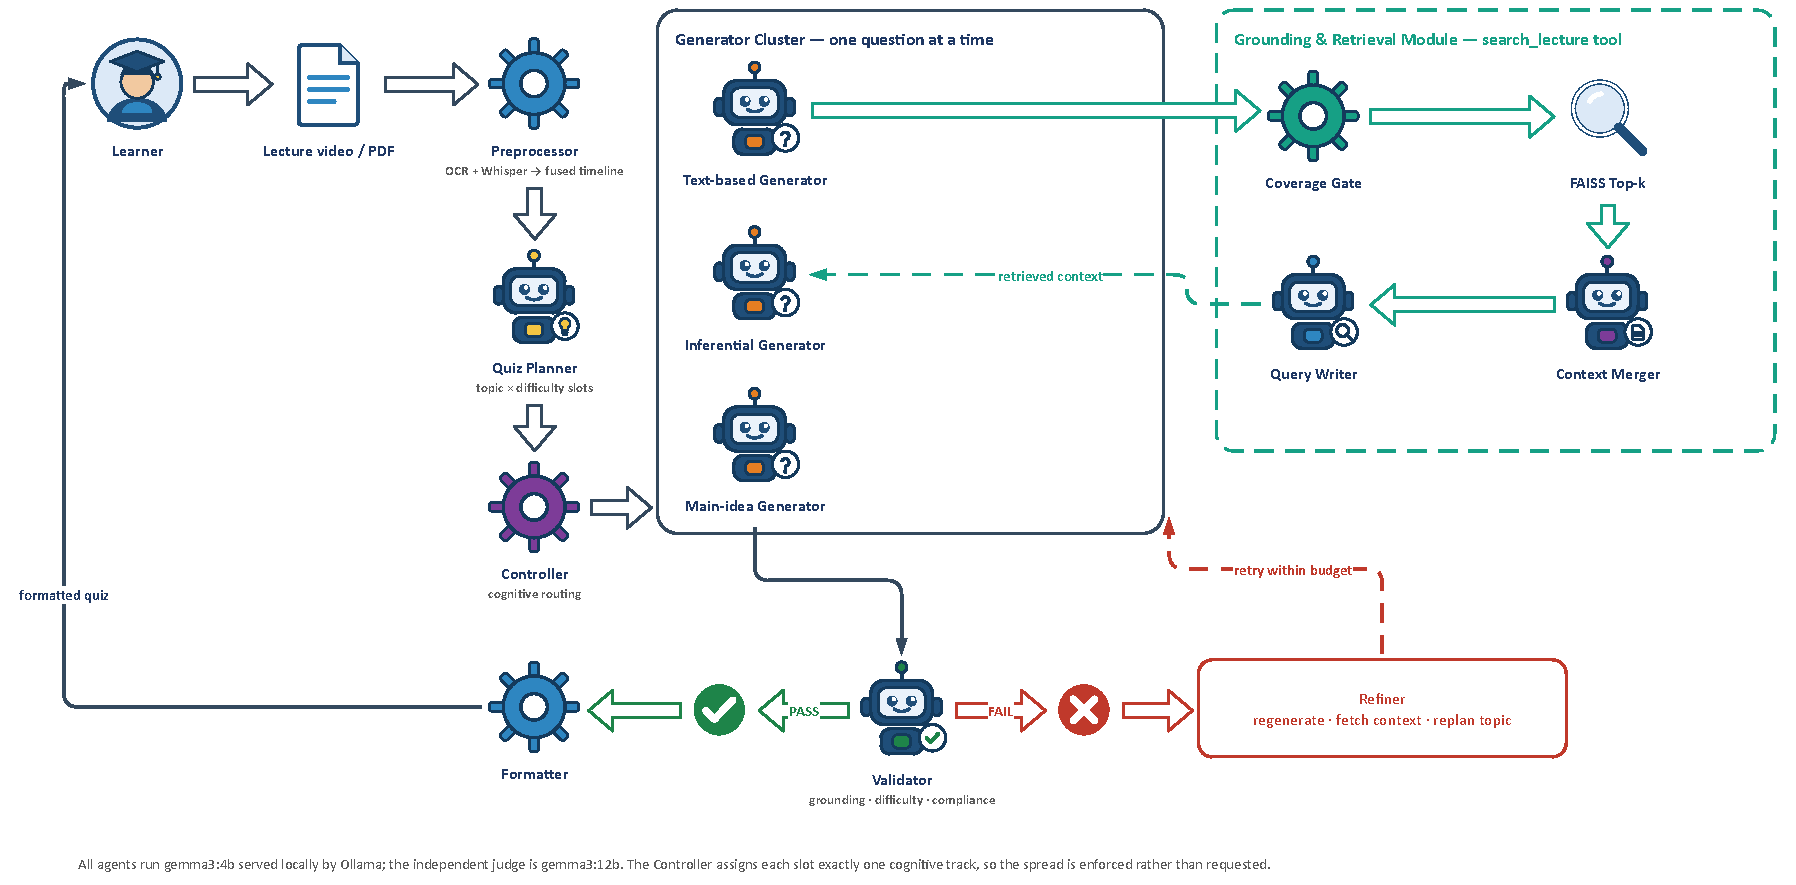
\includegraphics[width=\textwidth,height=30cm,keepaspectratio]{lectureassist-architecture-illustrated.pdf}
    \caption{System architecture of LectureAssist. The orchestrator coordinates
    specialist agents across ingestion, representation and generation: the
    Controller routes each slot to one of three cognitive tracks, the Validator
    accepts or rejects each drafted question, and a rejected question is
    diagnosed and returned to the Refiner rather than discarded. The dashed
    module on the right is the model-directed \texttt{search\_lecture}
    retrieval tool.}
    \label{fig:metho}
\end{figure}

\subsection{Data flow}
\label{sec:meth-flow}

The end-to-end flow is as follows.

\begin{enumerate}
  \item \textbf{Ingestion.} A video is sampled into frames and its audio track is
        demuxed; a document is parsed page by page.
  \item \textbf{Dual-channel extraction.} The visual channel goes to the
        \emph{Extractor} agent (scene-adaptive OCR); the audio channel goes to the
        \emph{Transcriber} agent (Faster-Whisper). Documents bypass both and go to
        the \emph{DocParser} agent.
  \item \textbf{Fusion.} OCR blocks and transcript segments are merged in
        timestamp order into a single unified lecture timeline, so that what the
        lecturer \emph{said} sits next to what they \emph{wrote} at the same moment.
  \item \textbf{Understanding.} The \emph{Summary} agent produces a structured
        summary; the \emph{RAG-Builder} agent chunks the content, embeds it and
        builds a vector index; the \emph{Hints} agent flags passages the lecturer
        marked as exam-relevant.
  \item \textbf{Generation.} The \emph{Quiz Planner} allocates questions across
        topics and difficulties; a \emph{Question Generator} drafts one question at
        a time; a \emph{Validator} accepts or rejects it and chooses a remediation
        action; a \emph{Refiner} applies it. This loop is the core of the system and
        is described in Section~\ref{sec:meth-agentic}.
  \item \textbf{Assessment and adaptation.} Answers are graded by a multi-tier
        grader; per-topic performance is written to a persistent profile, which the
        \emph{Adaptive Quiz} agent uses to bias the next quiz toward weak topics.
\end{enumerate}

\subsection{Scene-adaptive extraction}
\label{sec:meth-ocr}

A single OCR preprocessing recipe cannot handle a real lecture. White chalk on a
dark board is a low-contrast, inverted-polarity image; a projected slide in a lit
room is a bright, high-contrast one; a dark-theme slide deck looks superficially
like a blackboard but is destroyed by the inversion that a blackboard requires.
LectureAssist therefore \emph{classifies each sampled frame first} and preprocesses
it accordingly. Frames are routed by brightness and edge statistics into four
classes --- \texttt{slide}, \texttt{blackboard}, \texttt{whiteboard} and generic
\texttt{scene} (on-screen text) --- and each class gets its own contrast
enhancement, thresholding and, where appropriate, polarity inversion before being
passed to EasyOCR~\cite{easyocr}. Consecutive frames whose extracted text is more than $78\%$
similar are treated as the same board state and deduplicated, so that a slide left
on screen for two minutes contributes one block rather than sixty.

\subsection{Retrieval}
\label{sec:meth-rag}

Every generated artifact is grounded by retrieval-augmented
generation~\cite{lewis2020rag,gao2023ragsurvey}: the model is never asked to
recall the lecture from its weights, only to work from passages retrieved out of
the lecture itself.

The fused timeline is chunked and embedded with the Sentence-BERT
model~\cite{reimers2019sbert} \texttt{all-\allowbreak MiniLM-\allowbreak
L6-\allowbreak v2}~\cite{wang2020minilm}. The vectors are $L_2$-normalised and
indexed in FAISS~\cite{johnson2019faiss} with an inner-product index, so that
inner product equals cosine similarity (Eq.~\ref{eq:cosine}):
\begin{equation}
\label{eq:cosine}
\mathrm{sim}(q, c) \;=\;
  \frac{\mathbf{e}_q \cdot \mathbf{e}_c}
       {\lVert \mathbf{e}_q \rVert \, \lVert \mathbf{e}_c \rVert}
  \;=\; \hat{\mathbf{e}}_q \cdot \hat{\mathbf{e}}_c ,
  \qquad
  \hat{\mathbf{e}} = \frac{\mathbf{e}}{\lVert \mathbf{e} \rVert},
\end{equation}
where $\mathbf{e}_q, \mathbf{e}_c \in \mathbb{R}^{384}$ are the embeddings of the
query and of a candidate chunk. Because every vector is $L_2$-normalised before
insertion, the denominator is unity and a plain inner-product search returns exactly
the cosine ranking, which is why no separate normalisation step is needed at query
time. Retrieval returns the top
$k = 5$ chunks together with their timestamps, which is what allows both the chat
interface and a generated question to be traced back to the moment in the lecture
they came from. Crucially, retrieval is exposed to the generator agent as a
\emph{tool} (\texttt{search\_lecture}) rather than being applied unconditionally:
the agent decides for itself whether it needs more evidence.

\section{Hardware and/or Software Components}
\label{sec:meth-components}

The system is written in Python and served as a Flask~\cite{flask} API, with a single-page
HTML/JavaScript front end that talks to it over an ngrok~\cite{ngrok} tunnel; this split lets the
heavy models run on a Colab~\cite{colab} GPU while the interface runs in the student's own
browser. Table~\ref{tab:tools} lists the components, the alternatives considered,
and the reason for each choice. The overriding constraint throughout was that
\emph{nothing may require a paid API key}, since the target users are precisely
those for whom a per-token bill is prohibitive.

\begin{table}[H]
\centering
\caption{Software components, alternatives, and selection rationale.}
\label{tab:tools}
\footnotesize
\begin{tabular}{|p{2.6cm}|p{3.0cm}|p{3.2cm}|p{4.4cm}|}
\hline
\textbf{Tool} & \textbf{Function} & \textbf{Other similar tools} & \textbf{Why selected} \\
\hline
Gemma~3 (4B / 12B) & Generation, summarisation, grading, judging &
GPT-4, Claude, Llama~3, Mistral &
Open weights, runs locally, no API key; two sizes let the cheap model generate and
the strong model judge. \\
\hline
Ollama & Local LLM serving &
llama.cpp, vLLM, HF Transformers &
One-line model pull, automatic GPU offload, OpenAI-style local HTTP API; vLLM needs
more VRAM than a free T4 has. \\
\hline
Faster-Whisper (\texttt{small}) & Speech-to-text &
OpenAI Whisper API, Vosk, wav2vec2 &
Same accuracy as reference Whisper at a fraction of the memory; runs offline. The
API version is paid and cloud-bound. \\
\hline
EasyOCR (en, bn) & Board and slide text extraction &
Tesseract, PaddleOCR, Google Vision &
Deep-learning based, far better on handwriting than Tesseract; native Bengali
support matters for local lectures; Google Vision is a paid cloud API. \\
\hline
Sentence-Transformers \texttt{all-MiniLM-L6-v2} & Embeddings for RAG and for evaluation metrics &
OpenAI \texttt{text-embedding-3}, BGE, E5 &
$384$-dim, small and fast enough to co-exist with the LLM on one GPU; strong
quality-per-byte; local. \\
\hline
FAISS & Vector index &
Chroma, Pinecone, pgvector &
In-process, no server, no network; exact inner-product search is more than
sufficient at lecture scale. \\
\hline
PyMuPDF~\cite{pymupdf} & PDF/DOCX/PPTX parsing &
pdfplumber, PyPDF2 &
Fastest reliable text-layer extraction; preserves page structure used for
per-page source attribution. \\
\hline
Flask + ngrok & Backend API and public tunnel &
FastAPI, Gradio, Streamlit &
Minimal surface for a JSON API; ngrok exposes the Colab GPU to a browser UI running
on the student's own machine. \\
\hline
SymPy & Building the verified answer key for calibration &
Hand-computed answers, WolframAlpha &
Answers are \emph{machine-computed}, not hand-typed, so the calibration set cannot
inherit a human arithmetic error. \\
\hline
Google Colab (T4) + Drive & Compute and persistence &
Local GPU, RunPod, AWS &
Free tier is the realistic deployment target; Drive persistence lets a run survive
a runtime disconnect. \\
\hline
\end{tabular}
\end{table}

\section{Hardware and/or Software Implementation}
\label{sec:meth-impl}

\subsection{The agentic question-generation loop}
\label{sec:meth-agentic}

The agentic Question Generator produces \emph{one question at a time} through a
multi-stage loop. The design decision that distinguishes it from a
generate-then-filter pipeline is that the validator does not merely reject a bad
question --- it \emph{diagnoses} it and chooses how the next attempt should differ.
The stages are:

\begin{enumerate}
  \item \textbf{Plan.} The Quiz Planner reads the lecture summary and distributes
        the requested questions across the topics that are actually present, each
        with a target difficulty, yielding a list of (topic, difficulty) slots.
  \item \textbf{Retrieve.} Before drafting a slot, the generator inspects the content
        it holds and decides for itself whether it has enough material on that topic.
        If not, it issues its own retrieval query through the
        \texttt{search\_lecture} tool to pull more context. This is genuine tool use:
        the decision to retrieve is the model's, not a fixed step in the pipeline.
  \item \textbf{Generate.} It drafts exactly one question under a grounding rule ---
        the question must be answerable using only the supplied content --- rotating
        a question strategy on each attempt (concept-check, scenario,
        compare-and-justify) so that a retry is not merely a resample of the same
        prompt.
  \item \textbf{Validate.} A separate call checks the draft on three axes ---
        difficulty match, grounding, and instruction compliance --- and returns
        \texttt{PASS} or \texttt{FAIL} together with a remediation \texttt{action}.
  \item \textbf{Retry (loop back).} On \texttt{FAIL} the loop repeats within a retry
        budget, and the validator's chosen action decides the fix:
        \texttt{regenerate} (rewrite, with the failure reason fed back into the
        prompt), \texttt{fetch\_context} (retrieve more evidence first, then retry),
        or \texttt{replan\_topic} (abandon a topic that is not really in the lecture
        and swap to one that is).
  \item \textbf{Override.} If the retry budget is exhausted, the best attempt so far
        is kept and explicitly \emph{labelled} as an override. It is never silently
        recorded as a clean pass --- otherwise the pipeline's own accept rate would
        be a fiction.
\end{enumerate}

\begin{figure}[H]
\centering
\begin{tikzpicture}[x=1cm, y=1cm]

  % --- main chain -----------------------------------------------------------
  \node[laproc, text width=20mm] (plan) at (0,0)
       {Planner\\{\normalfont\scriptsize topic $+$ difficulty slots}};
  \node[lallm, text width=22mm]  (gen)  at (3.9,0)
       {Generator\\{\normalfont\scriptsize drafts ONE question}};
  \node[laval, text width=24mm]  (val)  at (8.1,0)
       {Validator\\{\normalfont\scriptsize grounding, difficulty, compliance}};
  \node[laout, text width=18mm]  (acc)  at (12.1,0)
       {Accept\\{\normalfont\scriptsize next slot}};

  % --- retrieval tool -------------------------------------------------------
  \node[latool, text width=34mm] (tool) at (3.9,2.15)
       {\texttt{search\_lecture}\\{\normalfont\scriptsize model-directed retrieval}};

  % --- remediation ----------------------------------------------------------
  \node[lallm, text width=53mm] (ref) at (8.3,-2.85)
       {Refiner\\{\normalfont\small the validator picks the fix}\\[1pt]
        {\normalfont\scriptsize \texttt{regenerate} $\;\cdot\;$
         \texttt{fetch\_context} $\;\cdot\;$ \texttt{replan\_topic}}};

  % --- edges ----------------------------------------------------------------
  \draw[laarr]  (plan) -- (gen);
  \draw[laarr]  (gen)  -- (val);
  \draw[laarrg] (val)  -- (acc) node[lalbl, midway, above]{PASS};
  \draw[laarrc] (tool) -- (gen)
        node[lalbl, midway, right]{evidence};
  \draw[laloop] (val.south) -- (ref.north)
        node[lalbl, midway, right]{FAIL};
  \draw[laloop] (ref.west) -| (gen.south)
        node[lalbl, pos=0.28, below]{retry $\leq 3$};
  \draw[laarr, draw=LAslate] (ref.south) -- ++(0,-0.75) -| (acc.south)
        node[lalbl, pos=0.30, below]
        {budget exhausted: keep best attempt, mark as override};

\end{tikzpicture}
\caption{The agentic question-generation loop. Questions are produced one at a time
and must pass validation before the next slot begins. The dashed edge is genuine
tool use: the generator decides for itself whether it has enough grounding and issues
its own retrieval query if not. On \texttt{FAIL} the validator does not merely
reject --- it selects the remediation, and only \texttt{regenerate} returns to the
generator directly, while \texttt{fetch\_context} and \texttt{replan\_topic} require
work outside the model first. When the retry budget is exhausted the best attempt is
kept but is explicitly labelled an override, so that a failure is never recorded as a
clean pass.}
\label{fig:agentic-loop}
\end{figure}

\subsection{Agent contracts and failure behaviour}
\label{sec:meth-contracts}

Every agent in the system inherits from a common base class and honours the same
four-stage contract: \texttt{should\_run}, which lets an agent decline work it
has no input for; \texttt{plan}, which records what it intends to do;
\texttt{execute}, which performs it; and \texttt{validate}, which checks its own
output before the orchestrator accepts it. The contract matters more than any
individual agent, because it is what makes the pipeline degrade rather than
fail: an agent that raises is caught by the orchestrator, its failure is written
to the agent log with the reason, and the remaining agents continue on whatever
context exists. A lecture whose audio track is unreadable still produces a
summary from board text alone.

Table~\ref{tab:agents} lists the agents, what each consumes and produces, and
what happens when it cannot do its job.

\begin{table}[H]
\centering
\caption{Agent contracts. Every agent validates its own output; the orchestrator
isolates failures so that one agent cannot abort the run.}
\label{tab:agents}
\footnotesize
\setlength{\tabcolsep}{4pt}
\begin{tabular}{|p{2.5cm}|p{3.1cm}|p{3.1cm}|p{4.0cm}|}
\hline
\textbf{Agent} & \textbf{Consumes} & \textbf{Produces} & \textbf{On failure} \\
\hline
Extractor & Video frames & Board and slide text, timestamped &
Run continues on audio alone \\
\hline
Transcriber & Audio track & Transcript segments with timestamps &
Run continues on board text alone \\
\hline
DocParser & PDF, DOCX, PPTX & Structured document text &
Run aborts; there is no other source \\
\hline
Summarizer & Fused timeline or document text & Structured summary &
Validated for length and refusal patterns, then retried \\
\hline
RAGBuilder & Summary and fused timeline & FAISS index over chunks &
Generation falls back to the summary without retrieval \\
\hline
Hints & Summary and timeline & Ranked exam-focus topics &
Planner falls back to summary topics \\
\hline
QuizPlanner & Summary, weak-topic profile & (topic, difficulty) slots &
Falls back to an even spread over summary topics \\
\hline
Quiz generator (Easy / Medium / Hard) & One slot, retrieved context &
One draft question & Retried under the loop of
Section~\ref{sec:meth-agentic} \\
\hline
QuizValidator & Draft question, accepted set & PASS/FAIL plus a remediation
action & A failed parse is treated as FAIL, never as PASS \\
\hline
QuizRefiner & Failed draft and its reason & Revised draft &
Loop falls back to plain regeneration \\
\hline
Answer generator & Question without the marked key & Independently derived
answer & Item is flagged unverified, not dropped \\
\hline
\end{tabular}
\end{table}

Two of these entries carry the project's central design commitments. The
validator treats an unparseable response as \texttt{FAIL} rather than
\texttt{PASS}, so a malformed reply can never inflate the acceptance rate; and
the answer generator's disagreement flags an item rather than deleting it, so
that the disagreement rate remains measurable instead of being silently
engineered away.

\subsection{Reproducibility and experimental control}
\label{sec:meth-repro}

Because the evaluation in Chapter~\ref{ch:results} compares two pipelines, the
things held constant between them matter as much as the thing varied. This
subsection records them.

\paragraph{Models are pinned, not chosen at run time.} The generator is
\texttt{gemma3:4b} and the primary model, used for summarisation, judging and
grading, is \texttt{gemma3:12b}; both are open-weight and served locally through
Ollama. The generator is \emph{pinned}: when it returns unusable structured
output the system retries the same model with a stricter instruction rather than
escalating to the larger one. Escalation would have been the better engineering
choice for output reliability, and it was deliberately rejected, because a
pipeline that silently falls back to a $12$B model when the $4$B model struggles
would no longer be measuring what it claims to measure. Every question in
Chapter~\ref{ch:results} was written by the model the chapter names.

\paragraph{Decoding parameters.} All calls use temperature $0.2$, a context
window of $16{,}384$ tokens, and an output ceiling of $8{,}192$ tokens. The low
temperature reflects the task: structured assessment items with a single defensible
key, not creative text. The output ceiling is a correctness requirement rather
than a tuning choice --- without it the server truncates generation at a few
hundred tokens, which silently cuts structured output mid-object and presents as
the generator having produced nothing.

\paragraph{Thresholds are fixed in advance.} The uniqueness check rejects a draft
whose similarity to any already-accepted question exceeds $0.85$; the retry
budget is three attempts per slot; frame de-duplication during extraction
suppresses consecutive frames above $0.97$ similarity; and short-answer grading
accepts a fuzzy match above $0.80$. These values were set before the evaluation
run and were not adjusted after seeing results.

\paragraph{What is \emph{not} controlled, and why it matters.} Generation is
sampled rather than greedy, and no random seed is fixed, so the run is not
bit-for-bit reproducible: repeating it produces a different question set with
similar statistics. This is a real limitation for exact replication and is
stated rather than hidden. It is mitigated by sample size, $200$ questions per
pipeline, and by the fact that the reported differences are consistent across
three difficulty strata rather than resting on a single aggregate. Fixing a seed
is a cheap improvement and is listed among the further work in
Section~\ref{sec:concl-future}.

\paragraph{The artifact trail.} Each run writes the generated questions, the
per-question validator verdicts with attempt counts and timings, and the full
agent decision log. Measurement is performed offline on those artifacts rather
than inside the generating session, so that scoring cannot influence generation
and so that a scoring change can be re-applied to an existing run without
regenerating it. The labelling correction disclosed in
Section~\ref{sec:res-native} is the one place where this separation proved
insufficient, and it is the reason a confirming re-run is the first item of
further work.

\subsection{The four generation pipelines}
\label{sec:meth-pipelines}

To isolate the contribution of the agentic machinery, the same content is used to
generate questions through four pipelines that differ \emph{only} in how the model
is asked:

\begin{itemize}
  \item \textbf{Agentic} --- the Plan $\rightarrow$ Retrieve $\rightarrow$ Generate
        $\rightarrow$ Validate $\rightarrow$ Retry loop of
        Section~\ref{sec:meth-agentic}.
  \item \textbf{Non-agentic (plain)} --- a single LLM call that emits the questions
        directly: no planning, no retrieval, no validation, no retry.
  \item \textbf{Chain-of-thought (CoT)} --- a single call in which the model must
        reason step by step to \emph{derive} each answer before committing to it,
        and record that reasoning.
  \item \textbf{Program-of-thought (PoT)} --- a single call in which the model must
        derive each answer through an explicit, ordered sequence of computation steps
        (define, substitute, simplify, evaluate) and mark the option equal to the
        final computed value.
\end{itemize}

CoT and PoT are both \emph{single-shot and non-agentic}: one LLM call, no
planning, retrieval, validation or retry. The only thing that separates them from the
plain baseline is the wording of the prompt. They emit the same JSON schema as the
plain generator, plus one extra field (\texttt{reasoning} or \texttt{computation})
that is retained for inspection but ignored by the downstream judge and Answer
Generator, so all four pipelines feed into an identical scoring path and are
directly comparable. The two prompts are reproduced verbatim below, since the
prompt \emph{is} the method.

Placeholders in square brackets are substituted at call time: \texttt{[N]} is the
requested question count, \texttt{[DIFF]} the target difficulty band (that line is
omitted entirely when no band is requested), and \texttt{[CONTENT]} and
\texttt{[SUMMARY]} the retrieved lecture text and its summary, truncated to $8000$
and $1500$ characters respectively. Line breaks are those of the prompt as sent;
where a line is too long for the page it wraps with a $\hookrightarrow$ marker.

\begin{lstlisting}[style=prompt,caption={Chain-of-thought generation prompt, as
sent to the generator. The reasoning field is recorded for inspection and is
ignored by the judge and the Answer Generator.},label={lst:cot}]
Generate [N] high-quality MCQ from this lecture content.
Difficulty focus: [DIFF]
Use CHAIN-OF-THOUGHT: for EACH question, think step by step to work out the correct answer BEFORE choosing it, and record that step-by-step reasoning. The option you mark correct MUST be exactly the answer your reasoning reaches, and each distractor must be wrong for a stateable reason.
STRICT JSON: {"questions":[{"question","options":{"A","B","C","D"},"reasoning","correct_answer","explanation","topic","difficulty","bloom_level","source_timestamp","source_type"}]}
'reasoning' = your step-by-step derivation of the correct option.

CONTENT:
[CONTENT]

SUMMARY:
[SUMMARY]
\end{lstlisting}

% Kept whole on one page: a prompt split across a page break is hard to read as
% a single artifact, and these two are meant to be compared line for line.
\newpage
\begin{lstlisting}[style=prompt,caption={Program-of-thought generation prompt.
Identical to Prompt~\ref{lst:cot} except for the reasoning instruction and the
name of the recorded field, so the two differ only in how the answer is required
to be derived.},label={lst:pot}]
Generate [N] high-quality MCQ from this lecture content.
Difficulty focus: [DIFF]
Use PROGRAM-OF-THOUGHT: for EACH question, derive the answer through an explicit ordered sequence of computation/derivation steps (like a short program: define, substitute, simplify, evaluate), record those steps, and only then mark the option that EQUALS the final computed result. The marked correct option MUST equal the endpoint of your computation.
STRICT JSON: {"questions":[{"question","options":{"A","B","C","D"},"computation","correct_answer","explanation","topic","difficulty","bloom_level","source_timestamp","source_type"}]}
'computation' = your ordered derivation steps ending at the correct value.

CONTENT:
[CONTENT]

SUMMARY:
[SUMMARY]
\end{lstlisting}

% \subsection{Controlling for confounds}
% \label{sec:meth-controls}

% Two implementation details are needed for the comparison to be fair, and both were
% bugs before they were features.

% \paragraph{Model pinning.} The generator is pinned to \texttt{gemma3:4b}. The
% original implementation silently escalated to the $12$B model whenever the $4$B
% returned malformed JSON, which would have made the claim ``these questions were
% written by the $4$B'' false for exactly the hardest questions --- the ones where the
% $4$B struggles. Pinning costs some yield and is required for an honest study.

% \paragraph{Content coverage.} A generator that only ever reads the first $8{,}000$
% characters of a $92{,}000$-character chapter can only ever ask about the first few
% pages, and will necessarily repeat itself. Each baseline therefore reads through a
% \emph{sliding window} over the document, and --- critically --- all three baselines
% use the same batch size, so they receive the same number of windows and see the same
% share of the chapter. Otherwise a pipeline that happened to use a smaller batch
% would read more of the document, and any difference in its questions would be
% confounded by content coverage rather than caused by the prompt. Likewise, the
% lecture summary that the planner uses to pick topics is produced by \emph{map-reduce}
% summarisation over the whole document rather than by truncating it, so the planner
% can propose topics from any part of the chapter.

\subsection{Answer correctness: two agents that must agree}
\label{sec:meth-answer}

A question can be well written and still mark the wrong option. Question generation
and answer generation are therefore treated as \emph{two distinct agents}, and their
answers are cross-checked. Correctness is measured three complementary ways:

\begin{itemize}
  \item \textbf{Independent re-solve (Answer Generator agent).} The larger model is
        given the stem and the options \emph{with the marked answer removed}, and
        solves the question from scratch. Its choice is compared with the Question
        Generator's marked answer; the agreement rate is the
        \emph{independent-match rate}. The solver never sees what it is supposed to
        agree with.
  \item \textbf{Judge-verify.} While scoring quality, the judge is additionally
        asked whether the marked answer is actually correct given the content,
        yielding the \emph{judge-verified-correct rate}. This is free --- it rides
        along on a call that was already being made.
  \item \textbf{Calibration on a known-answer set.} The generated questions have no
        ground-truth key, so neither of the above is an absolute measure of
        correctness --- if generator and solver share a misconception, they agree
        and are both wrong. To bound this, both models independently solve a set of
        MCQ whose answers \emph{are} known, and their accuracy on it calibrates how
        much the agreement rate above is worth. The calibration set is stratified
        into \emph{computational} items, whose answers are computed with
        SymPy~\cite{sympy} rather than typed by hand, and \emph{conceptual} items
        drawn from the chapter's definitions and theorems. This is reported
        separately and is explicitly \emph{not} a score on the generated questions.
\end{itemize}

The calibration set is used for evaluation only. It is never placed on the
generation path, since a generator that had seen the answer key would be scored on
questions it had effectively been given, and the resulting numbers would be
contaminated.

\subsection{System snapshot}
\label{sec:meth-snapshot}

Figures~\ref{fig:ui-workspace} and~\ref{fig:ui-quiz} show the deployed system in
use. They are included because the agentic loop described in
Section~\ref{sec:meth-agentic} is not only an internal mechanism: it is surfaced
directly to the user, and one of the design commitments of this project is that a
student should be able to see how a question was produced rather than being handed
an opaque result.

\begin{figure}[H]
\centering
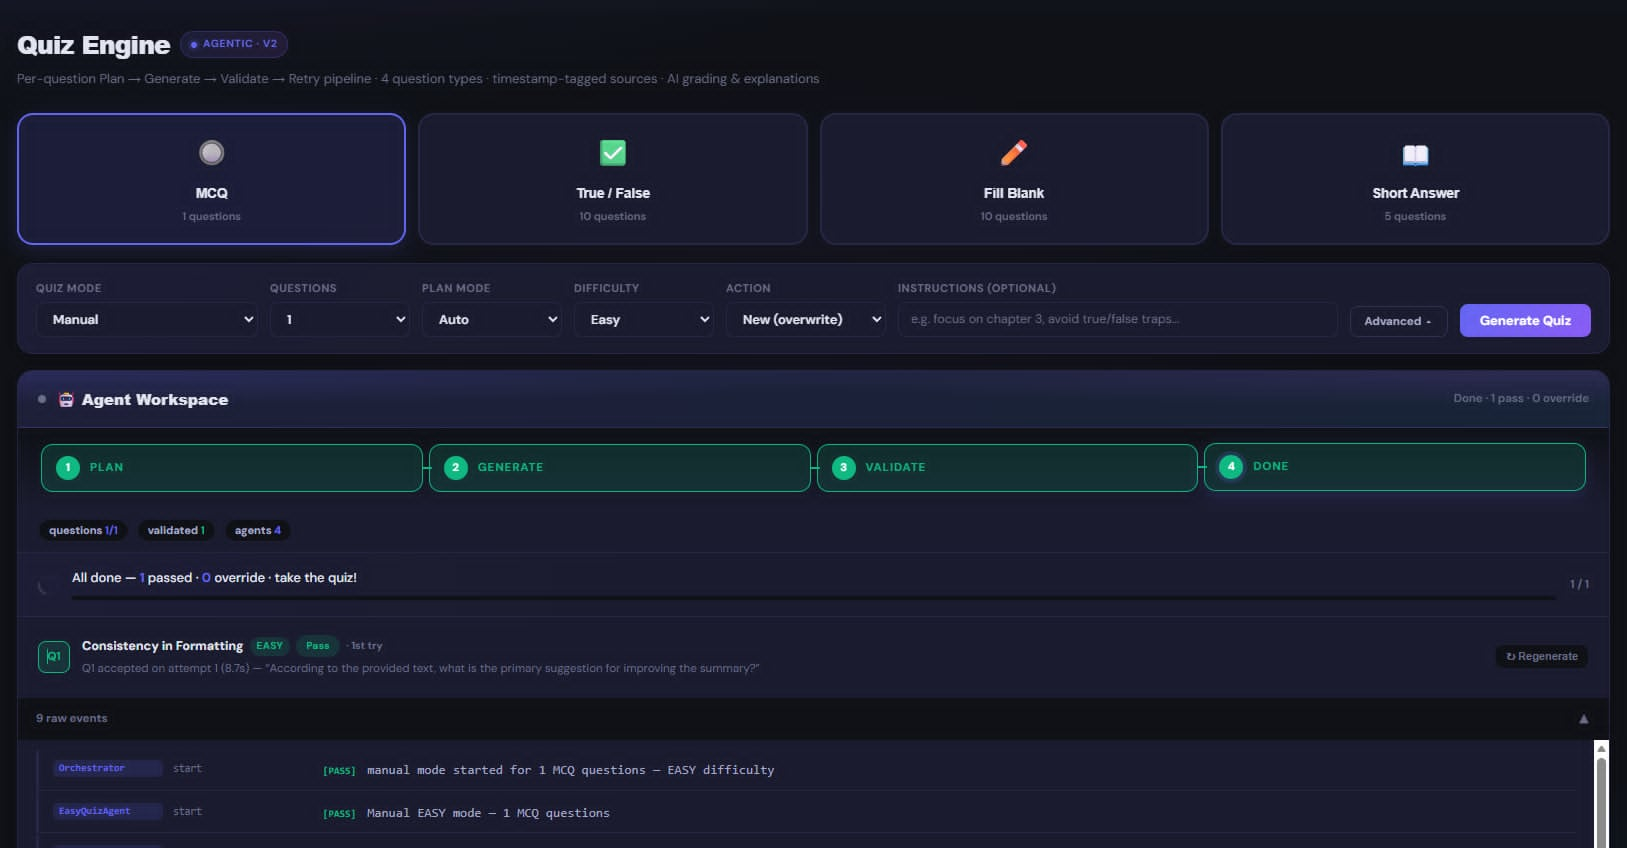
\includegraphics[width=\linewidth]{ui.jpg}
\caption{The Quiz Engine and its live Agent Workspace. The four stage indicators
across the top track the pipeline in real time as it runs. Beneath them, the counters
report questions completed, questions validated and agents active, and each generated
question appears as its own row recording the topic, the target difficulty, the
verdict, the attempt on which it was accepted and the time taken. The row shown here
was accepted on the first attempt in $8.7$ seconds. The raw event log at the bottom
names the agent responsible for every step, so a run can be audited after the fact
rather than inferred from its output.}
\label{fig:ui-workspace}
\end{figure}

\begin{figure}[H]
\centering
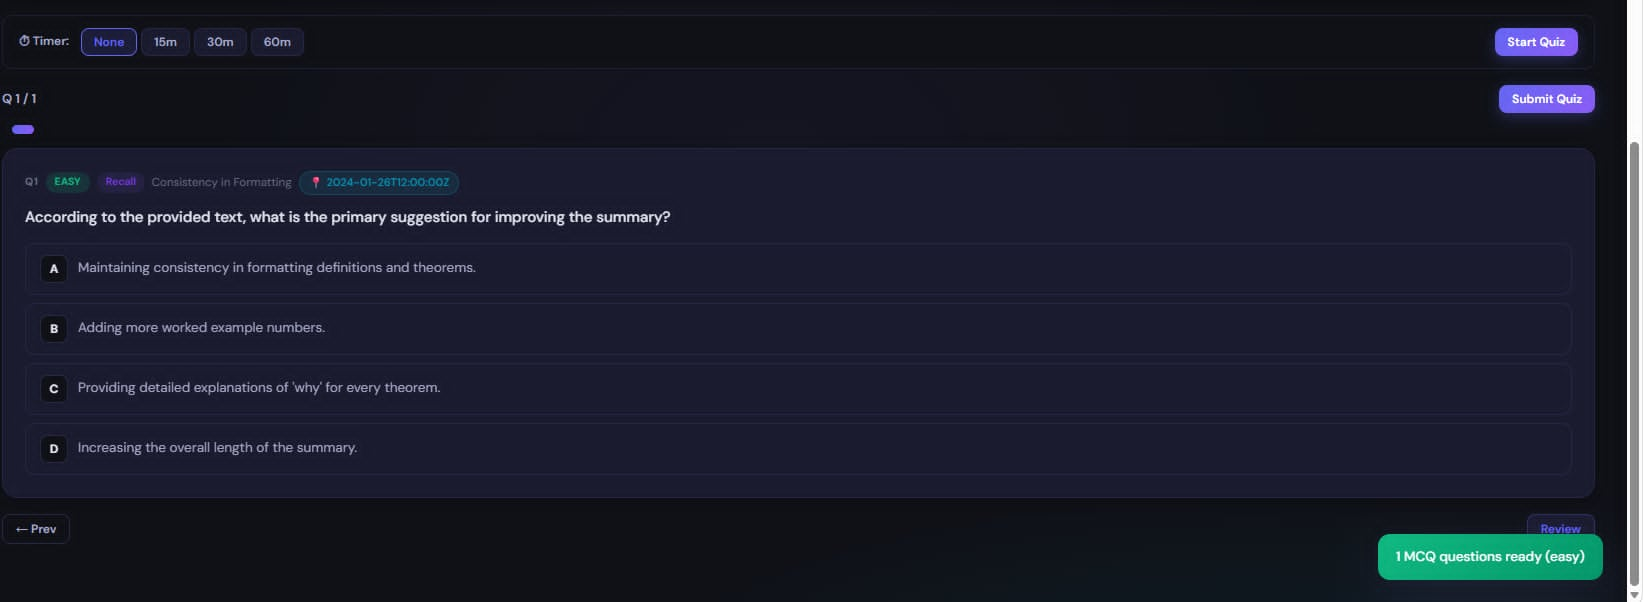
\includegraphics[width=\linewidth]{ui2.jpg}
\caption{The quiz-taking view. Each item carries its target difficulty, its Bloom
level and the topic it was planned against, together with the source timestamp of
the lecture material it was grounded in. That timestamp is what allows a student who
doubts an answer to return to the exact moment in the lecture the question came
from, which is the practical safeguard against the failure mode discussed in
Chapter~\ref{ch:impacts}.}
\label{fig:ui-quiz}
\end{figure}

\begin{figure}[H]
\centering
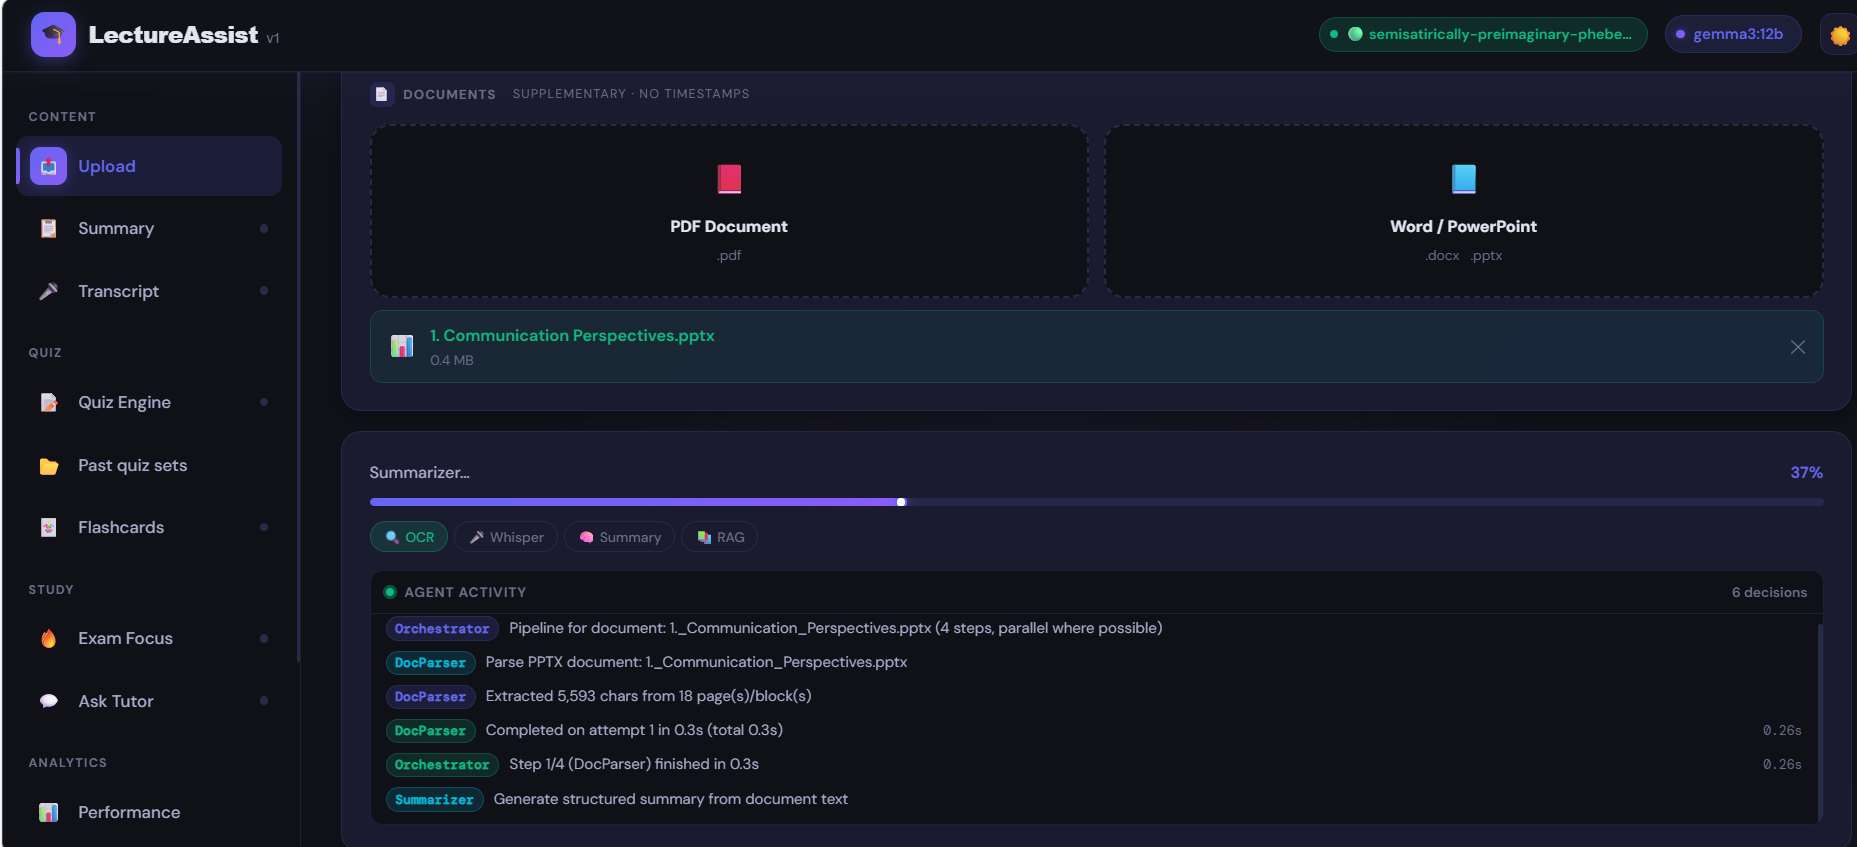
\includegraphics[width=\linewidth]{ui-upload-live.png}
\caption{Processing in progress. The agent activity feed streams each orchestrator
decision as it is taken rather than reporting them only once the run has finished:
the capture shows six decisions logged at $37\%$ completion, with the DocParser
having extracted $5{,}593$ characters from $18$ blocks in $0.3$ seconds and the
Summarizer already started. The stage pills above it track which of OCR, Whisper,
Summary and RAG is currently active.}
\label{fig:ui-live}
\end{figure}

\begin{figure}[H]
\centering
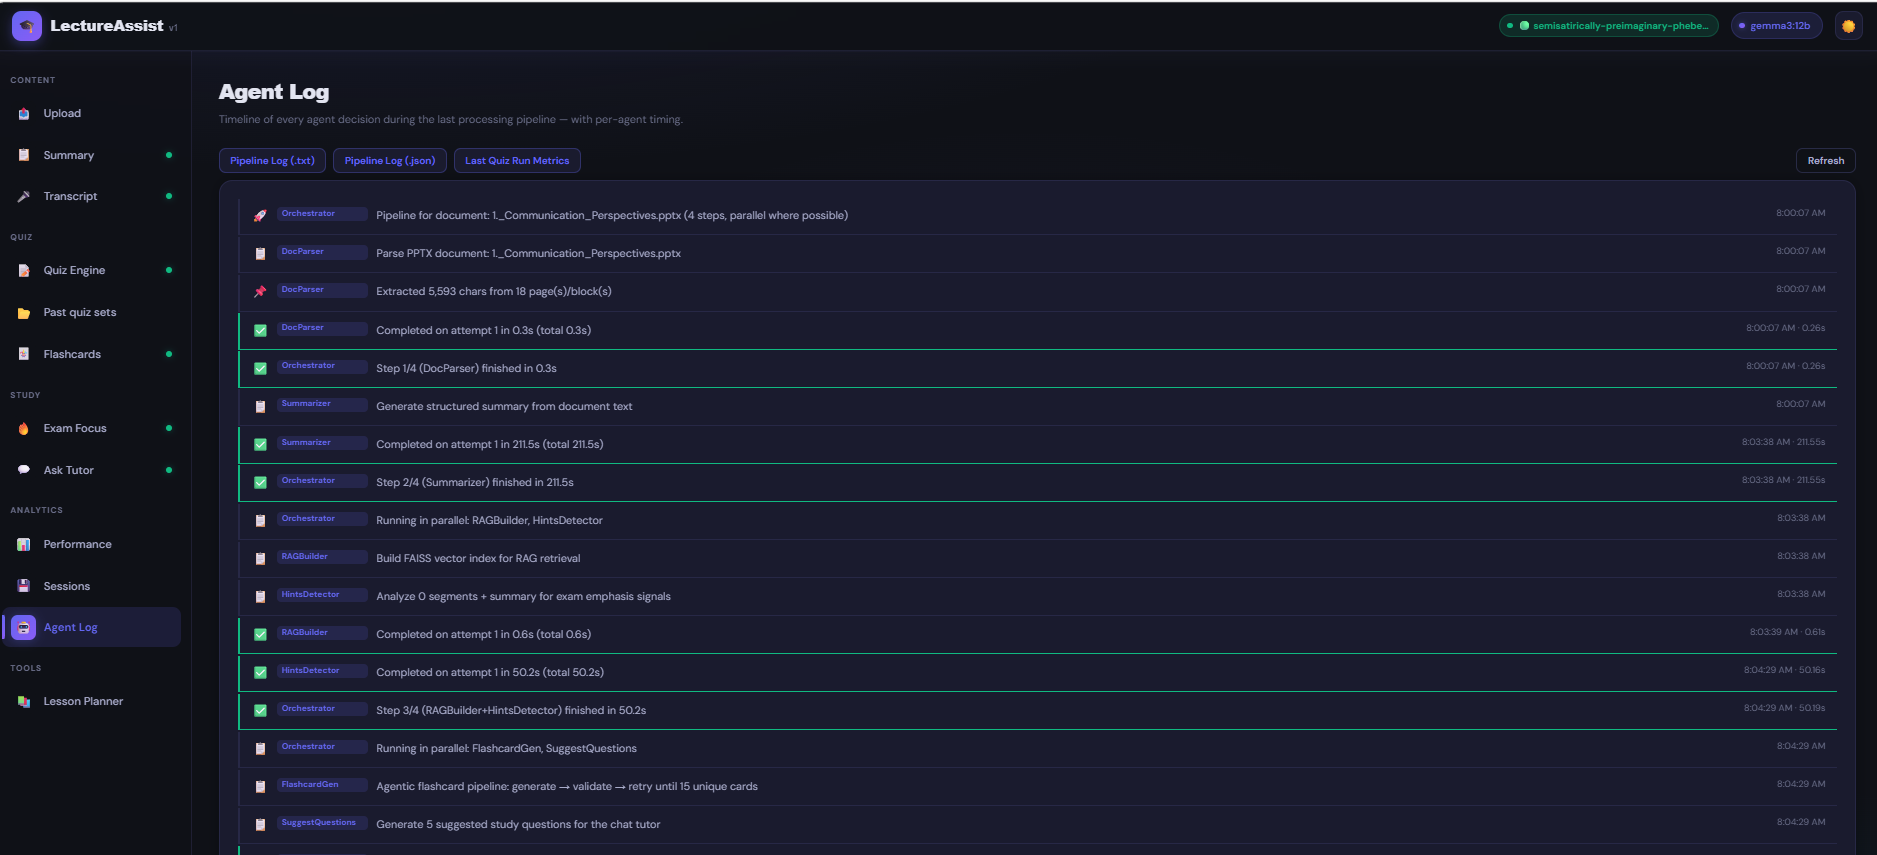
\includegraphics[width=\linewidth]{ui-agentlog.png}
\caption{The agent log for a completed document run, with per-agent timing. The
trail records not only which agent acted but how long each took and which steps the
orchestrator chose to run concurrently: DocParser completed in $0.3$s, the
Summarizer in $211.5$s, and RAGBuilder and HintsDetector were dispatched in parallel,
finishing in $0.6$s and $50.2$s respectively. The pipeline is therefore auditable
after the fact, which is what makes the timing claims in this chapter checkable
rather than asserted.}
\label{fig:ui-agentlog}
\end{figure}

\begin{figure}[H]
\centering
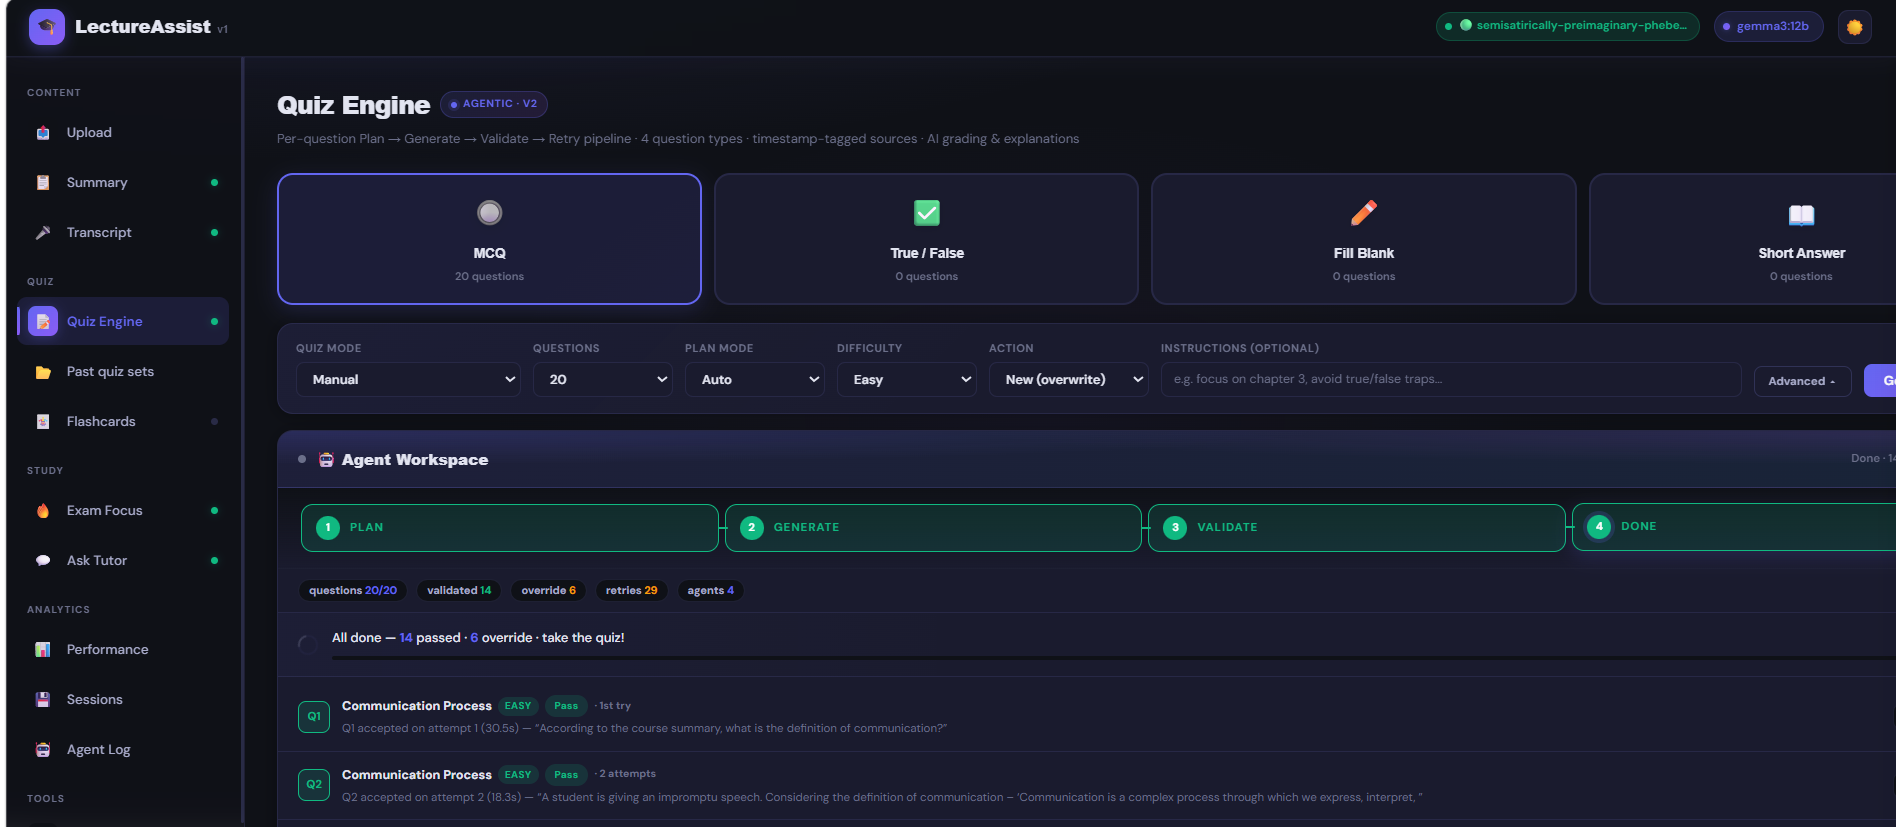
\includegraphics[width=\linewidth]{ui-quiz-run.png}
\caption{A full twenty-question generation. The counters read
\emph{questions $20/20$, validated $14$, override $6$, retries $29$, agents $4$},
and the status line states plainly that $14$ passed and $6$ were kept as overrides.
Twenty accepted questions therefore cost twenty-nine retries, which is the compute
multiplication discussed in Section~\ref{sec:impacts-economic} made visible.}
\label{fig:ui-quizrun}
\end{figure}

\begin{figure}[H]
\centering
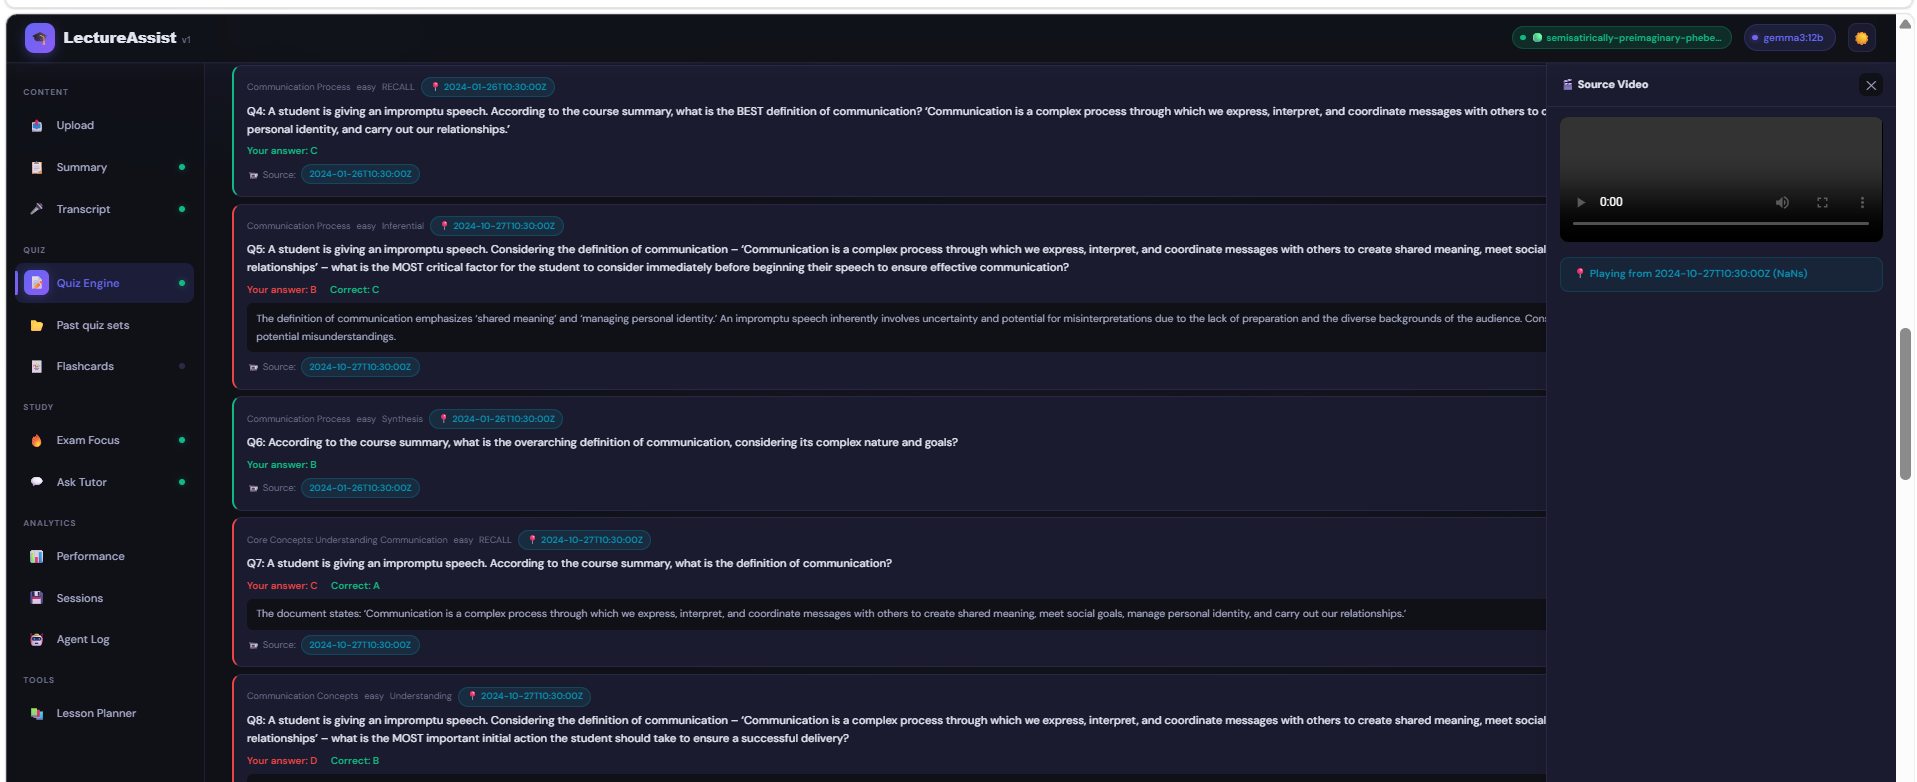
\includegraphics[width=\linewidth]{ui-graded.png}
\caption{The graded review, with the source panel open. Each item shows the marked
answer against the student's, the explanation drawn from the retrieved material, and
the lecture timestamp the question was grounded in; selecting that timestamp opens
the source at that moment. Items answered incorrectly are separated from those
answered correctly, so the review surface is also the input to the per-topic
weakness profile of Section~\ref{sec:meth-grading}.}
\label{fig:ui-graded}
\end{figure}

The counters in Figures~\ref{fig:ui-workspace} and~\ref{fig:ui-quizrun} distinguish
questions that passed validation from those kept as overrides, and
Figure~\ref{fig:ui-quizrun} is the more informative of the two because it is a run
in which overrides actually occurred: six of its twenty items exhausted the retry
budget. This distinction is shown rather than hidden for the reason given in
Section~\ref{sec:meth-agentic}: a pipeline that silently recorded an exhausted retry
budget as a clean pass would report an acceptance rate that was a fiction, and the
interface is built to make that impossible. The same figure is also the honest
counterweight to the loop's benefits, since it shows what the loop costs.

\subsection{Multi-tier grading and adaptation}
\label{sec:meth-grading}

Student answers are graded by a cascade chosen to match the question type. MCQ and
True/False are graded by exact key match. Fill-in-the-Blank is graded by a fallback
chain of exact match, then containment, then fuzzy string similarity above a $0.80$
threshold, so that a correct answer is not marked wrong over a typo or a plural.
Short Answer, where no string comparison is adequate, is graded by the $12$B model
against a rubric, which also returns concept-level feedback naming what the student
missed rather than merely marking it incorrect.

Every graded response updates a persistent per-topic profile. The Adaptive Quiz
agent reads that profile and biases the next quiz's topic and difficulty allocation
toward the topics where the student's accuracy is lowest, so that practice
concentrates where it is needed instead of being uniformly distributed.

\chapter{Investigation/Experiment, Result, Analysis and Discussion}
\label{ch:results}

This chapter reports the evaluation of LectureAssist's question generator. It
describes the environment the experiment was run in, defines the evaluation
protocol precisely, and reports the results. The evaluation adopts the protocol
of \textbf{EQGBench}~\cite{eqgbench}, a published benchmark for evaluating an
LLM's ability to \emph{generate} educational questions, so that the four
generation pipelines are scored on the same criteria a purpose-built
question-generation benchmark uses, rather than on ad-hoc metrics.

The experiment is designed around three questions.
\emph{RQ1:} judged on the EQGBench dimensions, does the agentic pipeline
produce better multiple-choice questions than single-shot prompting, including
the stronger chain-of-thought and program-of-thought prompting strategies?
\emph{RQ2:} how does each pipeline behave as the target difficulty rises from
easy to hard?
\emph{RQ3:} which dimensions actually separate the pipelines, and which
saturate?

\section{Environment Setup}
\label{sec:res-env}

Question \emph{generation} was run on a single Google Colab instance with an
NVIDIA T4 GPU ($16$\,GB), with models served locally by Ollama; no paid or
proprietary API is used anywhere in the generation path. Bulk-generation
artifacts are written to Google Drive so a run survives a Colab disconnection
and can be resumed rather than restarted.

The generator is \texttt{gemma3:4b}, pinned: it is never allowed to escalate to
a larger model, even when it returns malformed output, so that ``generated by
the $4$B'' is true of every question in the study.

\paragraph{Pipelines.} Four generation pipelines are compared, all using the
same pinned generator and the same source material:
\begin{itemize}
  \item \textbf{Agentic} --- the production per-question loop of
        \emph{Plan $\rightarrow$ Generate $\rightarrow$ Validate $\rightarrow$
        Retry}: a planner selects topics, each question is checked by a
        self-validator on grounding, difficulty, instruction compliance and
        uniqueness, and regenerated (with the failure reason fed back) until it
        passes or a retry budget is exhausted; the generator may issue its own
        retrieval query when it judges the supplied context insufficient.
  \item \textbf{Non-agentic} --- a single LLM call that writes questions
        directly, with no planning, validation, retrieval or retry.
  \item \textbf{Chain-of-thought (CoT)} --- as non-agentic, but the prompt
        instructs the model to reason step-by-step about the content before
        writing each question.
  \item \textbf{Program-of-thought (PoT)} --- as non-agentic, but the model is
        instructed to derive each question through explicit worked computation
        before committing to an answer.
\end{itemize}
The three baseline pipelines read the document through an identical sliding
window that steps across the whole chapter with a uniform batch size, so no
baseline is advantaged by seeing more or different content, and any difference
between them reflects the prompting strategy alone.

\paragraph{Source data.} Questions are generated from a college-level STEM
document --- the \emph{Limits} chapter of OpenStax \emph{Calculus, Volume~1}
\cite{openstax_calculus} --- ingested through the standard document pipeline
(extraction $\rightarrow$ map-reduce summary $\rightarrow$ retrieval index). The
extracted chapter text (about $112$k characters) is also supplied to the judge as
the ground-truth reference against which each question is scored
(Section~\ref{sec:res-protocol}).

\paragraph{Question corpus.} Each pipeline generated $50$ MCQs at each of three
target difficulties (easy, medium, hard). After generation, questions that were
structurally malformed (an empty option, or no valid A--D answer key) were
removed, since a malformed item cannot be judged fairly on any dimension. The
evaluated corpus is summarised in Table~\ref{tab:corpus}; the per-cell counts
$N$ are carried into every results table because they are not uniform.

\begin{table}[H]
\centering
\caption{Evaluated question corpus after removing structurally malformed items.}
\label{tab:corpus}
\small
\begin{tabular}{|l|c|c|c|c|}
\hline
\textbf{Pipeline} & \textbf{Easy} & \textbf{Medium} & \textbf{Hard} & \textbf{Total} \\
\hline
Agentic     & 49 & 44 & 40 & 133 \\
Non-agentic & 50 & 50 & 50 & 150 \\
CoT         & 50 & 50 & 50 & 150 \\
PoT         & 50 & 50 & 50 & 150 \\
\hline
\textbf{Total} & 199 & 194 & 190 & 583 \\
\hline
\end{tabular}
\end{table}

\section{Evaluation Protocol}
\label{sec:res-protocol}

The evaluation follows EQGBench~\cite{eqgbench}. Generation and measurement are
kept separate: the Colab run only \emph{generates} and saves every question to a
single JSON artifact; a standalone harness then reads that artifact and scores
each question. Scoring an already-generated corpus with a separate program means
the measurement can be repeated or re-judged without touching the system under
test.

\paragraph{Dimensions and scale.} Following EQGBench, every question is scored on
five dimensions, each on a three-point scale $\{0,1,2\}$ (Poor / Good /
Excellent):
\begin{itemize}
  \item \textbf{KP --- Knowledge-Point Alignment:} does the question genuinely
        target the intended knowledge point, grounded in the source material?
  \item \textbf{QT --- Question-Type Alignment:} is it a well-formed item of the
        requested type (a four-option MCQ with exactly one defensible answer)?
  \item \textbf{QQ --- Question Item Quality:} is the stem clear and
        unambiguous, and are the options and distractors well constructed?
  \item \textbf{SQ --- Solution Explanation Quality:} is the provided
        explanation correct, complete and pedagogically useful?
  \item \textbf{CG --- Competence-Oriented Guidance:} does the item cultivate
        understanding, reasoning or application (higher-order competence) rather
        than rote recall?
\end{itemize}
The reported per-pipeline score on each dimension is the mean over that
pipeline's questions, and the \emph{composite} is the mean of the five
dimensions.

\paragraph{Judge and voting.} EQGBench scores each question with a
reasoning-model judge and reduces judge noise by voting over repeated rounds.
The same procedure is used here: every question is judged \textbf{three times
independently}, and the final score on each dimension is the \emph{mode} of the
three rounds (the median is used on the rare occasion all three disagree). Each
judge call \emph{fails closed} --- a call that errors or returns unparseable
output contributes a zero, never an inflated score --- and a question whose three
rounds all fail is scored zero on every dimension rather than dropped.

\paragraph{Judge models.} EQGBench uses DeepSeek-R1 as its judge; that model was
not reachable through an accessible endpoint when this evaluation was run, so it
is not used here. Instead every question is scored by \emph{two} judges and both
are reported. The first is \texttt{gemma3:12b}, the larger local model, run
through the same offline harness; note that although it is a bigger model than
the \texttt{gemma3:4b} generator, it belongs to the same \texttt{gemma} family,
so it may share some of the generator's blind spots. The second is
\texttt{gpt-oss-120b}, a $120$B open-weight reasoning model from a different
family entirely, which serves as the cross-family check: where a same-family and
a cross-family judge agree, a pipeline's ranking cannot easily be dismissed as an
artifact of one model's quirks. Using two judges of different lineage --- and
reporting how far they agree --- is how this evaluation answers the objection
that an LLM judging an LLM's output is merely grading itself. What is adopted
from EQGBench is the \emph{protocol} --- the five dimensions, the $0$--$2$ scale,
and three-round voting --- not the specific judge model; results should be read
as EQGBench-protocol scores under these two independent judges.

\paragraph{Why not overlap metrics.} Following EQGBench, no $n$-gram overlap
metric (BLEU/ROUGE) is reported. Generation here is open-ended over a whole
chapter, so there is no reference question set to overlap with, and similarity
to any particular phrasing would not be evidence of quality.

\paragraph{Judge prompt.} Each question is sent to the judge with the source
material and the rubric below (reconstructed from the EQGBench dimension
definitions, as the benchmark has no public code release):

\begin{verbatim}
You are an expert evaluator of educational assessment items. Evaluate
this ONE multiple-choice question along the five EQGBench dimensions.
Score each dimension 0 (Poor), 1 (Good), or 2 (Excellent). Be strict;
2 is reserved for genuinely excellent performance on that dimension.

Reference material (ground truth): [chapter content]
Intended knowledge point (topic): [topic]
Requested question type: multiple-choice (4 options A-D, one correct)
Requested difficulty: [easy|medium|hard]

Question item:
Q: [question]      Options: [A-D]
Marked correct answer: [letter]
Provided solution explanation: [explanation]

Dimensions:
1. KP (Knowledge-Point Alignment)
2. QT (Question-Type Alignment)
3. QQ (Question Item Quality)
4. SQ (Solution Explanation Quality)
5. CG (Competence-Oriented Guidance)

Return STRICT JSON only:
{"KP":0,"QT":0,"QQ":0,"SQ":0,"CG":0}
\end{verbatim}

\section{Results and Discussion}
\label{sec:res-results}

\subsection{What EQGBench does}
\label{sec:res-what}

EQGBench is a published benchmark that asks a different question from most
evaluations. Instead of testing whether a model can \emph{answer} questions, it
tests whether a model can \emph{write} good educational questions. The authors
collected a large set of school-level science and mathematics material, asked
several large language models to generate questions from it, and then had a
strong ``judge'' model read each generated question and rate it. Every question
is rated on the five qualities listed earlier --- knowledge-point alignment,
question-type alignment, question quality, solution quality, and
competence-oriented guidance --- and each quality is given one of three grades:
poor, good, or excellent (written as $0$, $1$, and $2$). To keep a single
judge's opinion from dominating, each question is judged three times and the
grade that appears most often is kept.

The headline finding of EQGBench is the useful part for this project. On four of
the five qualities almost every model scored close to excellent, so those four
qualities did not tell the models apart. The fifth quality --- competence-oriented
guidance, that is, whether a question actually makes a student think rather than
just recall a fact --- was where every model scored poorly, and that is the
quality that separated the good models from the weak ones. Table~\ref{tab:eqg-their}
shows this pattern with figures reported in the EQGBench paper.

\begin{table}[H]
\centering
\caption{The pattern reported by EQGBench: the first four qualities are almost
maxed out for every model, while competence-oriented guidance (CG) collapses.
Figures are as reported in the EQGBench paper (mathematics subset) and are shown
to illustrate the pattern; exact values should be taken from the paper itself.}
\label{tab:eqg-their}
\small
\begin{tabular}{|l|c|c|}
\hline
\textbf{Quality (score out of 2)} & \textbf{Typical model} & \textbf{Pattern} \\
\hline
Knowledge-point alignment (KP) & $\approx 1.9$--$2.0$ & near-maximum for all \\
Question-type alignment (QT)   & $\approx 1.9$--$2.0$ & near-maximum for all \\
Question quality (QQ)          & $\approx 1.9$--$2.0$ & near-maximum for all \\
Solution quality (SQ)          & $\approx 1.9$--$2.0$ & near-maximum for all \\
Competence guidance (CG)       & $\approx 0.2$        & collapses for all \\
\hline
\end{tabular}
\end{table}

\subsection{How this fits our project}
\label{sec:res-fit}

Our system also \emph{writes} questions, so EQGBench is a natural fit: it was
built to measure exactly the task our generator performs. We therefore score our
four pipelines on the same five qualities, on the same three-point scale, using
the same three-times-and-take-the-most-common judging. This lets us report our
generator against an external, published yardstick rather than a scale we
invented ourselves.

Two honest differences should be stated plainly. First, EQGBench uses a specific
judge model (DeepSeek-R1); that model was not reachable when we ran our
evaluation, so we grade with two other strong models instead --- the local
\texttt{gemma3:12b} and a different-family reasoning model,
\texttt{gpt-oss-120b} --- and report both. Grading with two judges, one from the
same family as our generator and one from a different family, lets us show that a
result holds up no matter which judge is asked, rather than resting on a single
model's opinion. What we borrow from EQGBench is its method --- the five
qualities, the grading scale, and the repeated judging --- not its exact judge.
Second, EQGBench works on school-level science and mathematics, whereas our
questions come from a university calculus chapter; the method carries over, but
the subject matter is our own.

\subsection{How our evaluation works}
\label{sec:res-how}

The evaluation runs in two clearly separated stages. In the first stage the
system only \emph{generates}: all four pipelines produce their questions and
everything is saved to a single file, with no scoring involved. In the second
stage a separate program reads that file and does the scoring. Keeping the two
apart means the scoring can be repeated, or redone with a different judge, without
ever re-running or disturbing the generator.

For each saved question a judge is given the original chapter text as the source
of truth, together with the question, its options, its marked answer and its
explanation. The judge returns a grade of $0$, $1$ or $2$ on each of the five
qualities. This is repeated three times per question and the most common grade is
kept. If a judging attempt fails or returns something unreadable it is treated as
a zero rather than quietly ignored, so a broken question can never accidentally
look good. Each pipeline's score on a quality is simply the average of its
questions' grades, and its overall (composite) score is the average across the
five qualities. The whole scoring is then run a second time with the other judge,
so every pipeline ends up with a score from the local \texttt{gemma3:12b} and a
score from the different-family \texttt{gpt-oss-120b}, and the two can be compared.

\subsection{Our results}
\label{sec:res-ours}

Table~\ref{tab:eqg-overall} reports our four pipelines on the five qualities, and
Table~\ref{tab:eqg-bydiff} shows how the overall score changes with difficulty.
\emph{The judging run is still in progress; every cell shown as ``---'' is
pending, and no pending value has been filled in with an estimate.} Once the run
finishes, these tables are completed directly from the measured scores, and the
discussion below is written against the real numbers --- in particular, whether
our pipelines show the same pattern EQGBench found (the first four qualities
saturating while competence guidance separates them), and whether the agentic
pipeline's extra planning and checking earns it any advantage over plain, chain-of-thought
and program-of-thought prompting, especially on harder questions.

\begin{table}[H]
\centering
\caption{Our pipelines on the five EQGBench qualities (each out of $2$; composite
is the average of the five), judged three times per question, reported separately
for the two judges. Pending completion of the judging run; no value is estimated.}
\label{tab:eqg-overall}
\small
\begin{tabular}{|l|l|c|c|c|c|c|c|}
\hline
\textbf{Pipeline} & \textbf{Judge} & \textbf{KP} & \textbf{QT} & \textbf{QQ} &
\textbf{SQ} & \textbf{CG} & \textbf{Composite} \\
\hline
Agentic     & \texttt{gemma3:12b}   & --- & --- & --- & --- & --- & --- \\
            & \texttt{gpt-oss-120b} & --- & --- & --- & --- & --- & --- \\
\hline
Non-agentic & \texttt{gemma3:12b}   & --- & --- & --- & --- & --- & --- \\
            & \texttt{gpt-oss-120b} & --- & --- & --- & --- & --- & --- \\
\hline
CoT         & \texttt{gemma3:12b}   & --- & --- & --- & --- & --- & --- \\
            & \texttt{gpt-oss-120b} & --- & --- & --- & --- & --- & --- \\
\hline
PoT         & \texttt{gemma3:12b}   & --- & --- & --- & --- & --- & --- \\
            & \texttt{gpt-oss-120b} & --- & --- & --- & --- & --- & --- \\
\hline
\end{tabular}
\end{table}

\begin{table}[H]
\centering
\caption{Our overall (composite) score out of $2$ by difficulty, for each judge.
Pending completion of the judging run; no value is estimated.}
\label{tab:eqg-bydiff}
\small
\begin{tabular}{|l|l|c|c|c|}
\hline
\textbf{Pipeline} & \textbf{Judge} & \textbf{Easy} & \textbf{Medium} & \textbf{Hard} \\
\hline
Agentic     & \texttt{gemma3:12b}   & --- & --- & --- \\
            & \texttt{gpt-oss-120b} & --- & --- & --- \\
\hline
Non-agentic & \texttt{gemma3:12b}   & --- & --- & --- \\
            & \texttt{gpt-oss-120b} & --- & --- & --- \\
\hline
CoT         & \texttt{gemma3:12b}   & --- & --- & --- \\
            & \texttt{gpt-oss-120b} & --- & --- & --- \\
\hline
PoT         & \texttt{gemma3:12b}   & --- & --- & --- \\
            & \texttt{gpt-oss-120b} & --- & --- & --- \\
\hline
\end{tabular}
\end{table}

\section{Summary}
\label{sec:res-summary}

This chapter evaluated four question-generation pipelines --- agentic,
non-agentic, chain-of-thought and program-of-thought --- built on the same
pinned local \texttt{gemma3:4b} generator, using the EQGBench protocol: five
dimensions scored $0$--$2$, three-round voting, judged by two independent models
--- the local \texttt{gemma3:12b} and the different-family \texttt{gpt-oss-120b}.
The evaluation deliberately separates generation from measurement, scores an
already-generated corpus of $583$ questions, and reports per-cell sample sizes
because they are not uniform. The measured dimension
scores and the analysis of which dimensions discriminate between pipelines are
completed once the judging run finishes.

\chapter{Impacts and Design Constraints of the Project}
\label{ch:impacts}

This chapter examines the non-technical constraints that shaped LectureAssist,
economic, social, legal, ethical and environmental, and the impact the system
is likely to have once deployed. Several of the most consequential engineering
decisions in this project, notably the refusal to depend on any paid cloud
API, were driven by these constraints rather than by technical considerations.
They are therefore not an afterthought appended to a finished design; they are
among the inputs that produced it.

\section{Economic Impact}
\label{sec:impacts-economic}

\paragraph{The constraint that drove the architecture.} The system was
required to run without a paid API. This is not a stylistic preference, and it is
worth being precise about why. Per-token cloud pricing makes routine, high-volume
practice, which is precisely the usage pattern that makes retrieval practice
effective, prohibitively expensive for students in low- and middle-income
settings. It also makes the tool's availability contingent on a credit card and an
international payment rail that many students in Bangladesh and comparable settings
simply do not have; the barrier is not only the price but the mechanism of payment.
Every model in LectureAssist is therefore open-weight and locally served. The
consequence is a hard VRAM budget, which is why the generator is a $4$B model rather
than a frontier one, and much of the engineering documented in
Chapter~\ref{ch:methodology} exists to extract reliable structured output from a
small model. The evaluation in Chapter~\ref{ch:results} can be read as a test of
whether that constraint is survivable: it finds that a well-structured agentic loop
around a $4$B model measurably outperforms a single call to the same model, which is
the mechanism by which the cost constraint is absorbed rather than merely accepted.

\paragraph{Where the cost actually goes.} Removing the per-token bill does
not make the system free; it moves the cost from a recurring charge to a
one-off hardware requirement, and it is worth being clear about the trade.
A cloud deployment charges per question generated, so cost scales with
exactly the behaviour the system is trying to encourage: a student who
practises more pays more. Local inference inverts that. The marginal cost of
the thousandth question is the electricity to generate it, which means the
usage pattern that makes retrieval practice effective is the pattern the cost
model rewards. What replaces the bill is a floor: the system needs a GPU with
enough memory to hold a small generator and a larger judge, which in this
project is met by the free tier of a hosted notebook rather than by hardware
the student owns.

\paragraph{The compute cost of the agentic loop.} The architecture is not free
of economic consequence either. As Chapter~\ref{ch:results} records, the
five-agent pipeline costs roughly an order of magnitude more compute than the
single call it outperforms, because planning, retrieval, validation and retry
each add model invocations. On a paid API that multiplication is what makes
multi-agent decomposition expensive, and it is why the surveyed systems that
adopt it also depend on commercial inference. On local inference the same
multiplication costs time rather than money, which is the specific reason the
design is affordable here and would not be affordable in the cloud. The
ablation designs of Section~\ref{sec:res-ablation} exist partly to establish
whether the whole multiplication is necessary or whether a cheaper subset of
the agents captures most of the benefit, which is an economic question as much
as a scientific one.

\paragraph{Institutional adoption.} For a department rather than an individual,
the relevant comparison is against the staff time currently spent writing
practice items by hand. The system does not replace that work, because its
output is unreviewed until a human reviews it, but it changes the task from
authoring to checking. Whether that is a saving depends on how much of the
generated set survives review, and this project measures acceptance under an
automated judge rather than under an instructor, so the honest position is
that the institutional case is plausible but not evidenced here.

\section{Impact on Societal, Health, Safety, Legal and Cultural Issues}
\label{sec:impacts-society}

\paragraph{Educational and societal impact.} The core societal argument for
LectureAssist is one of access. Retrieval practice, repeatedly testing oneself on
material rather than re-reading it, is among the most effective study strategies
known, and the effect is large, replicated and long
established~\cite{roediger2006testenhanced,karpicke2011retrieval}. In the most
comprehensive review of study techniques available, practice testing is one of only
two techniques rated as having high utility across learners, materials and
criterion tasks~\cite{dunlosky2013improving}. Yet a supply of good practice questions
is a resource distributed very unevenly. A student at a well-resourced institution
has question banks, teaching assistants and instructor office hours; a student
without those has the end-of-chapter exercises and nothing else, and those exercises
are not tied to what their particular instructor actually emphasised in class. By
generating unlimited, validated, difficulty-controlled questions from the student's
\emph{own} lecture material, the system puts a form of practice that was previously a
privilege of well-resourced institutions within reach of anyone with a laptop. This
aligns directly with UN Sustainable Development Goal~4 (Quality Education) and,
because it removes a cost barrier rather than an ability barrier, with Goal~10
(Reduced Inequalities).

\paragraph{Safety: the risk of confidently teaching the wrong thing.} The most
serious safety issue in a system of this kind is not a crash: it is a fluent,
well-formed multiple-choice question whose marked answer is \emph{wrong}. A student
who trusts the tool will learn the error, rehearse it through exactly the retrieval
practice that makes the tool valuable, and carry it into an exam. The tool's fluency
works actively against their catching it, because the surface features a student uses
to judge whether a question is trustworthy, clear wording, plausible distractors,
a confident explanation, are precisely the features a language model produces most
reliably, whether or not the marked option is correct.

This risk shaped the evaluation methodology rather than merely being noted in it.
Answer correctness is measured separately from question quality, by an Answer
Generator agent that re-solves each question without ever seeing the marked option
(Section~\ref{sec:meth-answer}), and the solver is itself calibrated against
questions whose answers are known independently, so that its verdict is not
over-trusted. The honest conclusion is that the system's output is suitable for
\emph{practice} and must not be treated as an authoritative answer key. Any
deployment should surface this to the student directly, and no generated question
should be used for graded assessment without human review. The design implication is
concrete: the interface shows the source timestamp for every question, so that a
student who doubts an answer can jump to the moment in the lecture it came from
rather than having to trust or discard the question wholesale.

\paragraph{Legal and privacy considerations.} Lecture recordings and course materials
are frequently copyrighted by the instructor or the institution, and lecture audio
contains the identifiable voices of the instructor and, incidentally, of students who
ask questions. Uploading such material to a third-party cloud service to be processed, and potentially retained, logged, or used for training, raises copyright and
data-protection questions that most students are not in a position to evaluate, and
that they are typically not even prompted to consider. Because LectureAssist runs
entirely locally, the lecture never leaves the machine the user controls: there is no
third-party processor, and therefore no third-party retention. Users must still hold
the right to use the material they upload, and the system should not be used to
redistribute copyrighted lectures. The persistent per-topic performance profile is
educational data about an identifiable student, and it is stored in the user's own
storage rather than on any server operated by the developers.

One caveat must be recorded honestly. The evaluation deployment exposes the backend
through a public tunnel without authentication, as noted in
Section~\ref{sec:concl-limits}. That is acceptable for a supervised demonstration and
is not acceptable for real use, and it is the first thing that would have to change
before the system were put in front of students.

\paragraph{Cultural and linguistic considerations.} OCR is configured for both
English and Bengali, reflecting the reality of instruction in Bangladesh, where
lecturers routinely switch languages mid-sentence and write on the board in either.
A pipeline that only read English would silently discard part of the lecture, and
would do so invisibly, since a missing board block looks exactly like a board that
was never written on. This is a recurring theme in the system's failure modes: the
dangerous errors are the ones that produce no error, and the design response is to
widen coverage rather than to detect absence, because absence in this pipeline is
undetectable in principle.

\section{Ethical Considerations}
\label{sec:impacts-ethics}

Ethical questions arise for this system in two distinct registers, and it is
worth separating them. The first concerns the conduct of the research itself:
what this report claims, and on what evidence. The second concerns the artifact:
what a deployed question generator can do to the people who rely on it. The
safety and privacy dimensions of the second register are treated in
Section~\ref{sec:impacts-society}; this section addresses the commitments and
obligations that follow from them.

\subsection{Research Ethics}

Two ethical commitments governed this work, and both are visible in the
structure of Chapter~\ref{ch:results}.

\paragraph{No fabricated results.} Every number reported in
Chapter~\ref{ch:results} comes from a measured run, and the report claims
nothing beyond what was measured. It would have been easy to present a fuller
looking set of results by supplying plausible values for comparisons that were
designed but not carried out; that option was rejected, and the chapter reports
the comparison that was actually run and analyses it thoroughly instead. The
limitations of those measurements, particularly the saturation of the judged
dimensions and the weakness of an LLM solver as a proxy for correctness, are
stated plainly rather than omitted because they are unflattering. Where a labelling correction had to be applied
that cannot be re-derived from the stored artifacts, that fact is disclosed in
the results chapter and again in the limitations, rather than quietly
incorporated.

\paragraph{No misrepresentation of the system's capability.} The tool is an
aid to practice, not a substitute for the instructor or the textbook, and this
report is explicit about where its output cannot be trusted. A system that
generates assessment material carries a specific professional obligation not
to overstate its reliability, because the people most likely to over-trust it
are precisely the students with the least access to an expert who could
correct them: the same students the system is built for.

\subsection{Ethics of Deployment}

\paragraph{Academic integrity.} A system that turns a lecture into questions can
also be turned toward producing answers, and the boundary between the two is
thinner than it looks. LectureAssist is deliberately built as a
\emph{self-assessment} instrument: it generates questions for a student to
attempt, grades the attempt, and reports which topics were weak. It does not
draft submittable coursework, and the short-answer grader returns feedback
against the lecture rather than a polished answer to be copied. That boundary is
a design decision rather than a technical impossibility, and it is stated here so
that it is understood as a commitment which any future extension of the system
inherits. An instructor adopting the tool should also be told what it is: an
item generator whose output is unreviewed until a human reviews it.

\paragraph{The obligation created by confident error.} The safety analysis in
Section~\ref{sec:impacts-society} establishes that a fluent, wrong question is
the characteristic failure of this class of system. The ethical consequence is
that the burden of detection cannot be placed on the learner, because a student
who could reliably detect a subtly wrong question about a topic would not need
to be tested on it. This is why answer correctness is checked by a second agent
that never sees the marked option, why items that fail validation are flagged as
overrides rather than silently accepted, and why every generated item carries a
timestamp back to the source so a doubt can be resolved against the lecture
rather than against the model. These are ethical requirements expressed as
architecture, and they are the reason for design choices that would otherwise
look like unnecessary cost.

\paragraph{Data, consent and ownership.} Lecture recordings contain the voice,
and often the image, of an instructor who has not consented to third-party
processing, and the material itself is usually the instructor's or the
institution's intellectual property. Running entirely on local inference is the
strongest available mitigation, because the recording is never transmitted to a
provider who could retain it, train on it, or be compelled to disclose it. The
legal dimension is treated in Section~\ref{sec:impacts-society}; the ethical
point is narrower and applies even where the law is silent: a student's right to
study a lecture they attended does not extend to redistributing their
instructor's teaching, and the system should not make redistribution the path of
least resistance. Retention is correspondingly limited to what a session needs.

\paragraph{Bias, coverage and who the system serves.} Two kinds of bias bear on
this system. The first is inherited: the generator, the judge and the
independent solver are all language models trained on corpora that
over-represent English and well-resourced academic domains, so question quality
will not be uniform across subjects or languages, and this report offers no
evidence about performance outside the single English STEM chapter evaluated in
Chapter~\ref{ch:results}. The second is structural and specific to the
evaluation: the judge and the solver are drawn from the same model family as the
generator, so they share its blind spots, and agreement between them is evidence
of consistency rather than of correctness. That limitation is stated in
Chapter~\ref{ch:results} as a measurement caveat; it is repeated here because it
is also an ethical one. A system that grades itself with a model like itself
will systematically fail to detect the errors that model is prone to, and it
should not be presented to students as an independent check on their
understanding.

\paragraph{Boundaries of responsible use.} Taken together, the commitments above
define what this system may honestly be claimed to do. It is a practice and
revision aid, grounded in a specific lecture, whose output is checked but not
guaranteed. It is not an examination instrument, not a substitute for the
instructor, and not a source of authority about the subject matter. Deploying it
in any of those three roles would exceed what the evaluation in
Chapter~\ref{ch:results} supports, and the project treats that as an ethical
limit rather than a marketing one.

\section{Impact on Environment and Sustainability}
\label{sec:impacts-env}

The environmental footprint of an AI system is dominated by the energy consumed
during inference at scale. LectureAssist's design happens to be favourable on this
axis, largely as a side effect of the constraint that it must run on a free-tier GPU.

\paragraph{Small models, local inference.} Question generation runs on a
$4$B-parameter model rather than a frontier-scale one, and the entire system runs on
a single consumer GPU. Inference on a small local model consumes orders of magnitude
less energy per request than routing that request to a hyperscale data centre running
a model two to three orders of magnitude larger, and it avoids the network transfer
and data-centre cooling overhead entirely. No model was trained or fine-tuned during
this project, all models are used as released, so the substantial carbon cost
of training was not incurred by this work.

\paragraph{Caching and resumability as energy savings.} OCR results are cached and
keyed by a hash of the video, so re-processing the same lecture costs nothing.
Consecutive frames whose extracted text is more than $78\%$ similar are treated as
one board state, so a slide left on screen for two minutes contributes one block
rather than sixty. Bulk evaluation runs are checkpointed to persistent storage so
that a disconnection resumes rather than restarts. Each of these was implemented for
practical reasons, free-tier compute is scarce and Colab runtimes die, but each
also directly avoids recomputing work that has already been done, which is the
cheapest energy saving available and the only one that costs nothing in quality.

\paragraph{The honest counterweight: the agentic loop is not free.} The agentic
pipeline consumes substantially more compute than a single-shot baseline, because it
issues a planning call, up to three drafting calls, a validation call per attempt,
and any retrieval calls the generator elects to make, against the baseline's one.
Chapter~\ref{ch:results} finds that this buys a real and consistent quality
improvement on every metric that discriminates, so the expenditure is not wasted.
But ``not wasted'' is a weaker claim than ``efficient'', and the report should not
pretend otherwise. This is exactly why every ablation and merging table in
Chapter~\ref{ch:results} carries a mandatory cost column: a configuration that
matches the full pipeline's quality using two-thirds of the calls is
environmentally as well as economically preferable, and the experiment is designed so
that such a configuration would be identified rather than overlooked. Reducing the
call count at fixed quality is simultaneously a performance goal, a cost goal and an
environmental one, and the three do not conflict.

\paragraph{Sustainability of access.} A tool that requires a subscription is
sustainable only for as long as the student can pay for it, and only for as long as
the vendor chooses to keep that model available at a stable price. Models are
deprecated, prices change, and free tiers are withdrawn. Because LectureAssist
depends on no external service, it will continue to work on hardware a student
already owns, for as long as they own it, with weights they have already downloaded.
This is an important form of sustainability that is easy to overlook when
sustainability is framed purely in terms of energy consumption: a system that stops
working when a company changes its pricing has a lifespan measured in business
decisions rather than in hardware.

\chapter{Project Planning and Budget}
\label{ch:planning}

This chapter documents how the project was planned and resourced. It sets out the
development methodology, decomposes the work into a structured breakdown, presents
the thirty-week schedule as a Gantt chart with explicit milestones, assigns
responsibility across the team, records the risks that were identified and how they
were mitigated, and closes with the project budget. A recurring theme throughout is
that the schedule and the budget were shaped by the same constraint that shaped the
architecture: the system had to be buildable and runnable on free-tier hardware with
no paid inference service.

\section{Development Methodology}
\label{sec:plan-method}

The project followed an \emph{incremental, artifact-driven} methodology rather
than a strict waterfall or a fixed-sprint agile process. This choice was
forced by the nature of the system. LectureAssist is a pipeline in which each
stage consumes the output of the previous one, and several of those stages,
optical character recognition, speech transcription, bulk question generation,
are expensive enough that they cannot be re-run casually on a free-tier GPU.
The pipeline was therefore built stage by stage, and each stage was required
to emit a \emph{durable, inspectable artifact} to persistent storage before
the next stage was started.

Three consequences followed from that decision, and all three shaped the schedule
visible in Section~\ref{sec:plan-gantt}.

\paragraph{Stages could be developed and debugged independently.} Because the OCR
stage writes a cached, hashed transcript of every board state to disk, the retrieval
stage could be developed against that cached file without re-running OCR even once.
This is why the extraction tasks and the retrieval task overlap in the schedule
rather than running strictly in series.

\paragraph{Expensive work became resumable.} A Colab runtime disconnection is not an
exceptional event on the free tier; it is a routine one. Checkpointing every
generation and judging run to Google Drive converted a class of failure that would
otherwise have cost days of re-computation into one that costs minutes. Without this,
the bulk evaluation task in weeks 24--27 would not have been feasible at all inside
the schedule.

\paragraph{Measurement was decoupled from generation.} Generation and scoring were
deliberately implemented as separate programs communicating through a JSON artifact
on disk. This meant the evaluation harnesses could be written, corrected and re-run
against an already-generated corpus without regenerating a single question, which
is precisely what happened when the first EQGBench protocol implementation was
judged unfaithful to the published prompt and had to be rewritten.

\section{Work Breakdown Structure}
\label{sec:plan-wbs}

The project was decomposed into five phases containing twenty work packages. Phases
correspond to coherent subsystems rather than to calendar periods, which is why they
overlap in time. Table~\ref{tab:wbs} lists them with their deliverables.

{\footnotesize\singlespacing
\setlength{\tabcolsep}{4pt}
\begin{longtable}{|l|p{5.0cm}|p{5.6cm}|c|}
\caption{Work breakdown structure. Each work package produces a deliverable that a
later package consumes.}
\label{tab:wbs}\\
\hline
\textbf{WP} & \textbf{Work package} & \textbf{Deliverable} & \textbf{Weeks} \\
\hline
\endfirsthead
\hline
\textbf{WP} & \textbf{Work package} & \textbf{Deliverable} & \textbf{Weeks} \\
\hline
\endhead
\hline
\endfoot
\hline
\endlastfoot

\multicolumn{4}{|l|}{\emph{Phase 1, Planning and Research}} \\
\hline
1.1 & Literature review & Annotated bibliography; research gap & 1--5 \\
1.2 & Requirement analysis and scope & Functional requirement list & 2--4 \\
1.3 & Toolchain selection, environment setup & Working Colab + Ollama runtime & 4--6 \\
\hline
\multicolumn{4}{|l|}{\emph{Phase 2, Multimodal Extraction}} \\
\hline
2.1 & Frame sampling and scene classification & Four-class frame router & 5--8 \\
2.2 & Scene-adaptive OCR & Deduplicated board-text blocks & 7--11 \\
2.3 & Speech transcription & Timestamped transcript segments & 8--10 \\
2.4 & Timeline fusion and document parsing & Unified lecture timeline & 10--12 \\
2.5 & Retrieval index construction & FAISS index; \texttt{search\_lecture} tool & 11--13 \\
\hline
\multicolumn{4}{|l|}{\emph{Phase 3, Agentic Generation Pipeline}} \\
\hline
3.1 & Agent framework and orchestrator & \texttt{BaseAgent}; agent event log & 12--15 \\
3.2 & Planner and Generator agents & Topic--difficulty slots; drafted items & 14--17 \\
3.3 & Validator and Refiner loop & Verdict plus remediation action & 16--19 \\
3.4 & Five question types; multi-tier grading & Grading cascade; feedback & 18--21 \\
3.5 & Adaptive difficulty engine & Persistent per-topic profile & 20--22 \\
\hline
\multicolumn{4}{|l|}{\emph{Phase 4, Interface and Integration}} \\
\hline
4.1 & Flask API and tunnel deployment & Public JSON API & 15--18 \\
4.2 & Web interface and live agent workspace & Single-page front end & 17--22 \\
4.3 & End-to-end integration and debugging & Demonstrable system & 21--24 \\
\hline
\multicolumn{4}{|l|}{\emph{Phase 5, Evaluation and Documentation}} \\
\hline
5.1 & Evaluation harnesses & Three scoring programs & 22--26 \\
5.2 & Bulk generation and judging runs & Scored question corpus & 24--27 \\
5.3 & Ablation and merging experiments & Per-agent attribution & 26--28 \\
5.4 & Report, poster and defence & This report; A0 poster & 25--30 \\
\hline
\end{longtable}
}

\section{Project Schedule}
\label{sec:plan-gantt}

Figure~\ref{fig:gantt} presents the thirty-week schedule. The project spans two
academic terms: CSE~499A covers weeks 1--15 and CSE~499B covers weeks 16--30, marked
on the chart by the vertical divider. The division is not merely administrative. By
the end of week 15 the system had to be able to take a lecture video and produce a
grounded, retrievable representation of it; everything that generates, validates or
evaluates questions depends on that representation existing and was therefore
scheduled after it.

\begin{figure}[H]
\centering
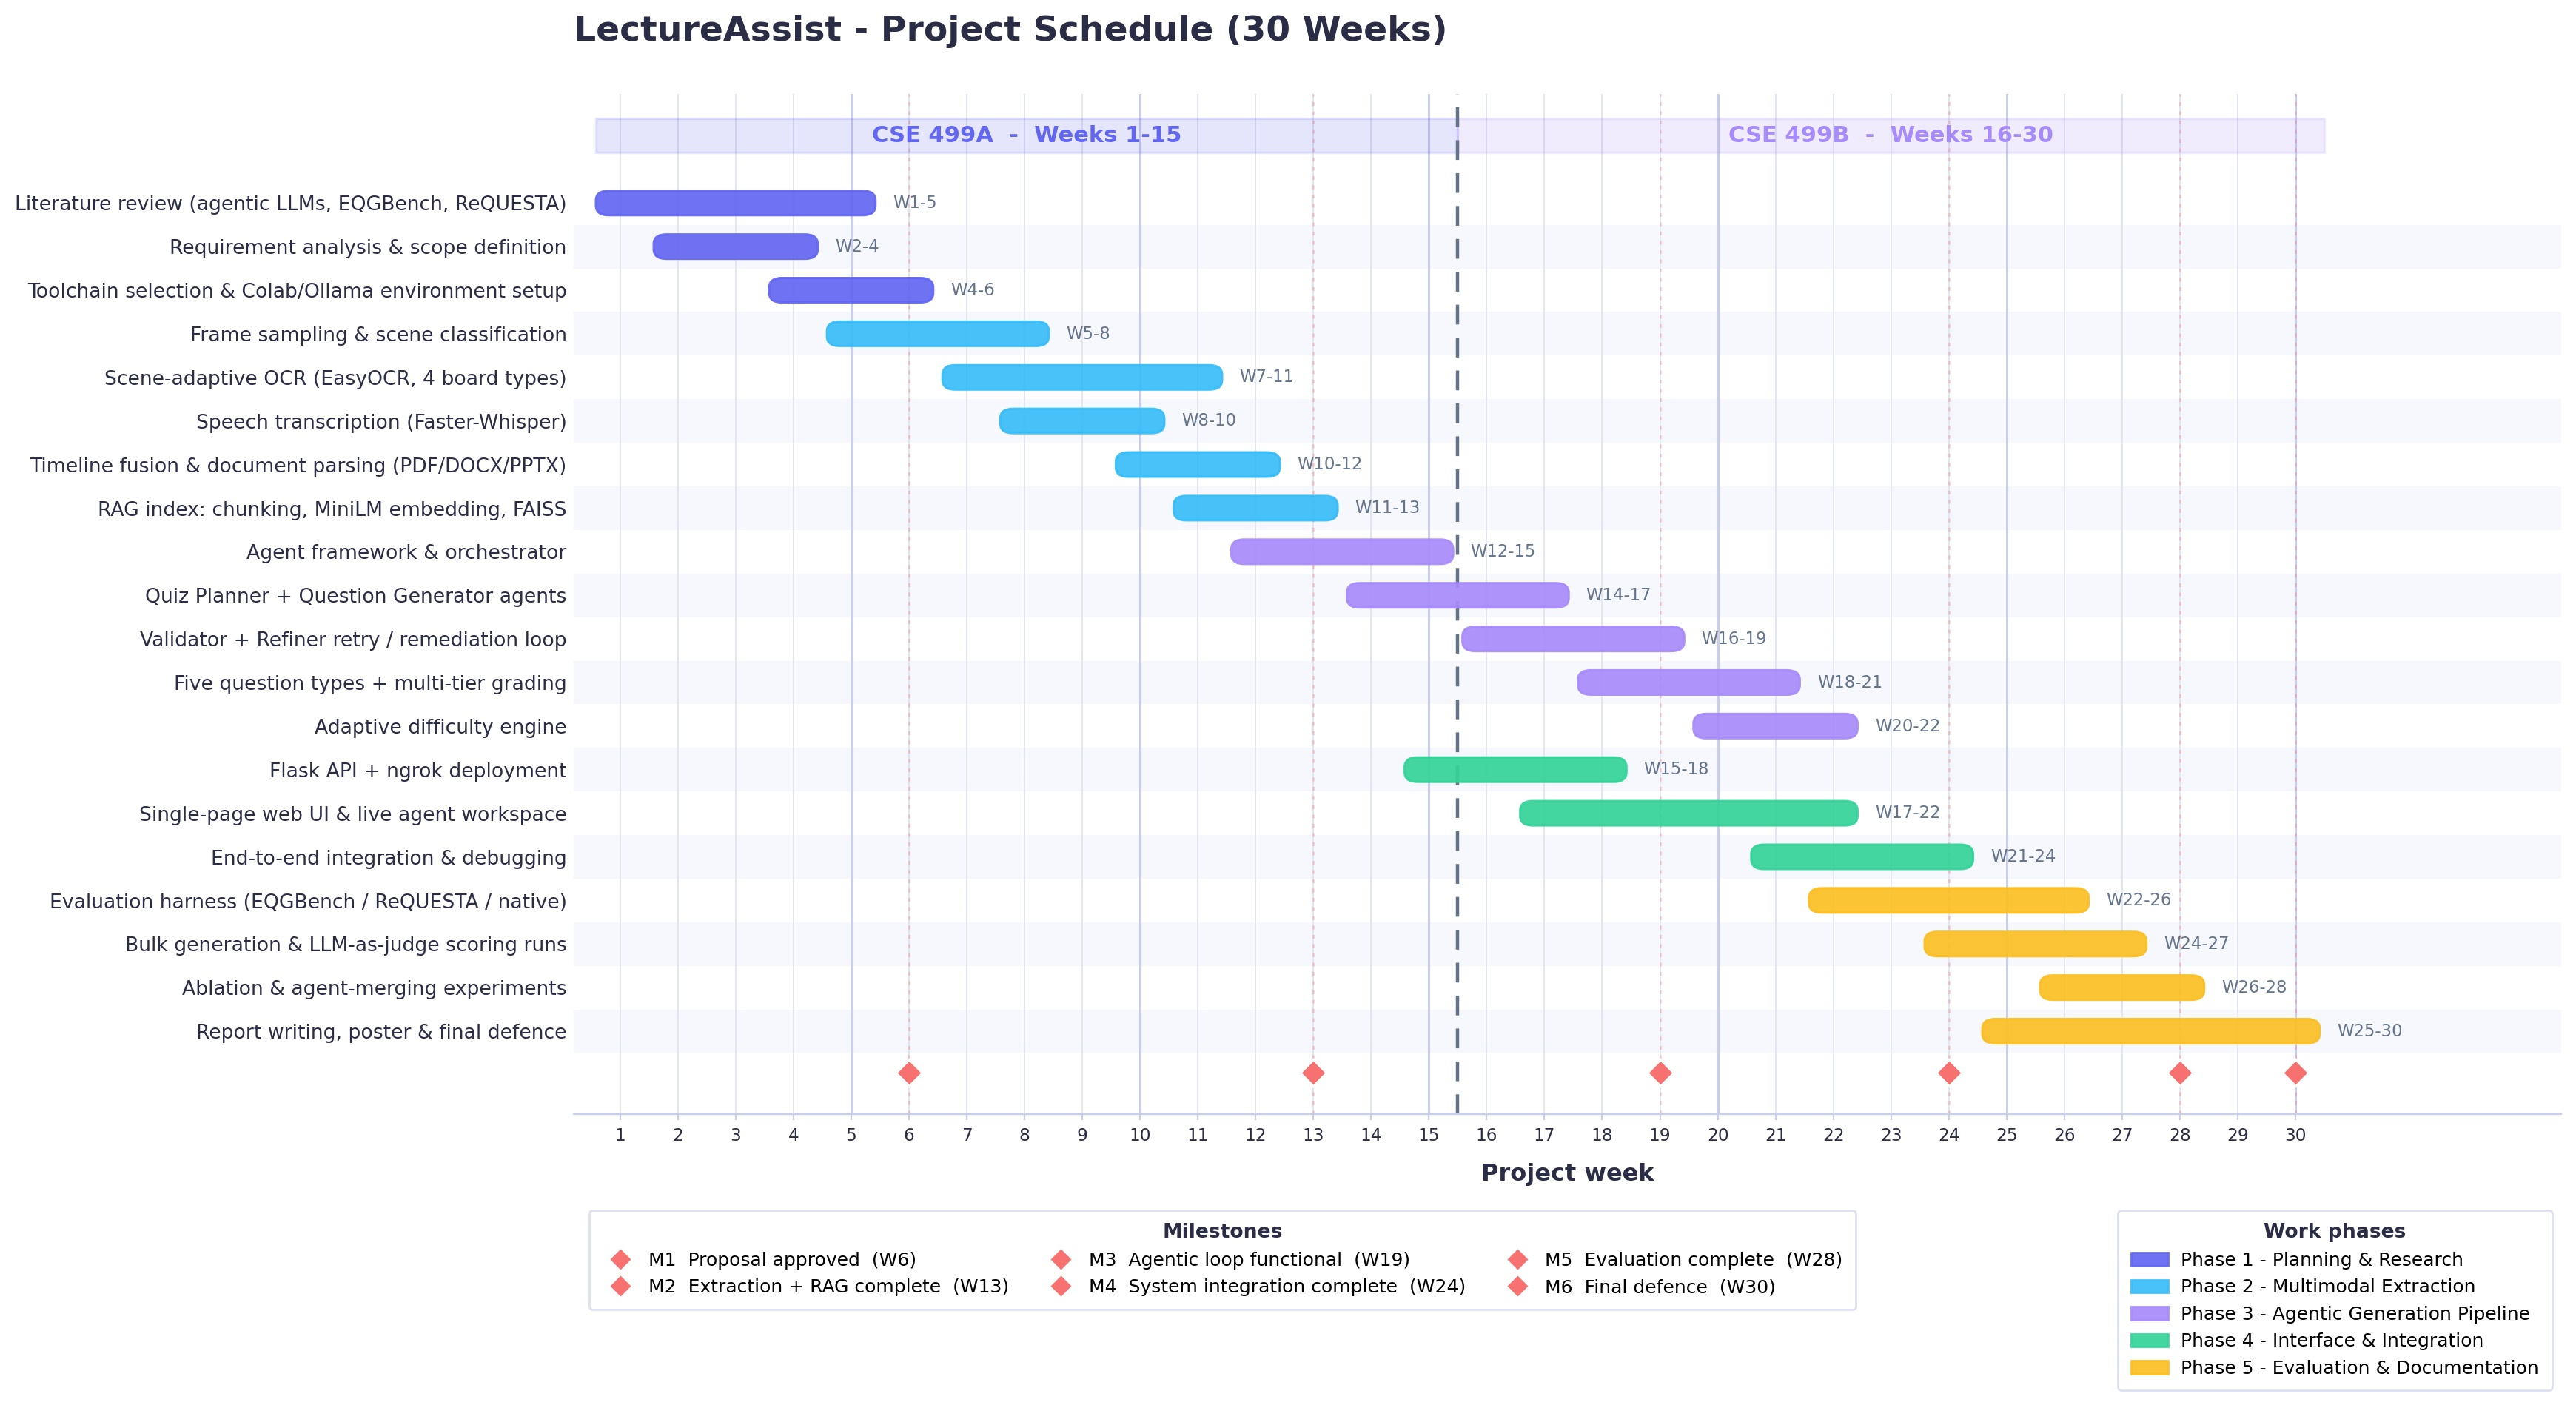
\includegraphics[width=\linewidth]{gantt_chart.jpg}
\caption{Project schedule across thirty weeks, showing twenty work packages grouped
into five phases, the CSE~499A/499B term boundary at week 15, and six milestones.
Overlapping bars reflect the artifact-driven methodology of
Section~\ref{sec:plan-method}: a downstream stage begins as soon as the upstream
stage emits a usable artifact, not when it is finished.}
\label{fig:gantt}
\end{figure}

Three scheduling decisions in that chart are worth justifying explicitly, because
each represents a deliberate trade-off rather than a default.

\paragraph{Extraction and retrieval overlap.} Work package 2.5 begins in week 11,
while OCR work package 2.2 is still running. This was possible only because of the
caching decision described above, and it bought roughly two weeks of slack that were
later consumed by the evaluation phase.

\paragraph{The interface was built early and in parallel.} Front-end work begins in
week 17, well before the pipeline was complete. The reasoning was that the live agent
workspace, which visualises the per-question Plan, Generate, Validate and Retry
trace as it happens, is not merely a presentation layer but a debugging instrument.
Having it available during weeks 18--21 materially accelerated the development of the
validator and refiner, because a failing remediation decision could be seen directly
rather than reconstructed from logs.

\paragraph{Evaluation was given eight weeks, and needed them.} Weeks 22--30 are
dominated by measurement rather than construction. This allocation was made after the
first pilot judging run showed that a faithful implementation of a published protocol
is considerably more work than it appears: EQGBench requires five separate judging
calls per question, repeated over three independent rounds, and ReQUESTA turned out
to publish no judge prompt at all. Both harnesses had to be written from the papers
themselves rather than adapted from released code.

\begin{table}[H]
\centering
\caption{Project milestones and their acceptance criteria.}
\label{tab:milestones}
\footnotesize
\begin{tabular}{|c|c|p{4.2cm}|p{5.4cm}|}
\hline
\textbf{ID} & \textbf{Week} & \textbf{Milestone} & \textbf{Acceptance criterion} \\
\hline
M1 & 6  & Proposal approved &
     Scope, research gap and toolchain agreed with the supervisor \\
M2 & 13 & Extraction and retrieval complete &
     A lecture video yields a fused, timestamped, retrievable timeline \\
M3 & 19 & Agentic loop functional &
     A question is planned, drafted, validated and remediated end to end \\
M4 & 24 & System integration complete &
     All five question types, grading and adaptation reachable from the interface \\
M5 & 28 & Evaluation complete &
     Bulk corpus generated and scored; metrics computed from a real run \\
M6 & 30 & Final defence &
     Report submitted, poster printed, system demonstrated live \\
\hline
\end{tabular}
\end{table}

\section{Team Roles and Responsibilities}
\label{sec:plan-raci}

The team consists of three members working under one supervisor.
Responsibility was assigned per work package using a RACI allocation,
Responsible, Accountable, Consulted, Informed, reproduced in
Table~\ref{tab:raci}. In every row exactly one member is Accountable, so that
no work package could be left un-owned.

{\footnotesize\singlespacing
\setlength{\tabcolsep}{5pt}
\begin{longtable}{|p{5.4cm}|c|c|c|c|}
\caption{RACI responsibility matrix. R = Responsible (does the work),
A = Accountable (owns the outcome), C = Consulted, I = Informed.}
\label{tab:raci}\\
\hline
\textbf{Work package} & \textbf{Iftikhar} & \textbf{Salman} & \textbf{Jarinah}
 & \textbf{Supervisor} \\
\hline
\endfirsthead
\hline
\textbf{Work package} & \textbf{Iftikhar} & \textbf{Salman} & \textbf{Jarinah}
 & \textbf{Supervisor} \\
\hline
\endhead
\hline
\endfoot
\hline
\endlastfoot

Literature review and research gap      & R & C & A & C \\
Requirement analysis and scope          & C & A & R & A \\
Extraction: OCR and scene classification & A & R & C & I \\
Extraction: speech transcription        & R & A & C & I \\
Timeline fusion and document parsing    & A & C & R & I \\
Retrieval index and search tool         & C & A & R & I \\
Agent framework and orchestrator        & R & A & C & C \\
Planner, Generator, Validator, Refiner  & C & A & R & C \\
Question types and grading cascade      & A & R & C & I \\
Adaptive difficulty engine              & R & C & A & I \\
Flask API and deployment                & A & R & I & I \\
Web interface and agent workspace       & R & I & A & I \\
Evaluation harnesses                    & C & A & R & C \\
Bulk runs and result analysis           & R & A & C & C \\
Report, poster and defence              & R & R & R & A \\
\hline
\end{longtable}
}

\section{Risk Management}
\label{sec:plan-risk}

Table~\ref{tab:risks} is the risk register maintained across the project. It is
reproduced here as it was used rather than as a retrospective idealisation, which is
why it includes risks that materialised. Likelihood and impact are rated on a
three-point scale (L/M/H).

{\footnotesize\singlespacing
\setlength{\tabcolsep}{4pt}
\begin{longtable}{|p{3.6cm}|c|c|p{6.4cm}|c|}
\caption{Risk register. Risks marked \emph{occurred} were realised during the
project and were handled by the stated mitigation.}
\label{tab:risks}\\
\hline
\textbf{Risk} & \textbf{L} & \textbf{I} & \textbf{Mitigation} & \textbf{Status} \\
\hline
\endfirsthead
\hline
\textbf{Risk} & \textbf{L} & \textbf{I} & \textbf{Mitigation} & \textbf{Status} \\
\hline
\endhead
\hline
\endfoot
\hline
\endlastfoot

Colab runtime disconnects mid-run &
  H & H &
  Checkpoint every artifact to Drive after each question; make all long runs
  resumable rather than restartable &
  occurred \\
\hline
Free-tier GPU memory insufficient for both the LLM and the embedding model &
  M & H &
  Pin generation to the 4B model; use a 384-dimension embedding model that
  co-exists with it; keep the 12B model for judging only &
  occurred \\
\hline
The 4B generator returns malformed JSON &
  H & M &
  A staged JSON repair chain (escape fixing, quote normalisation, block slicing)
  followed by retry on the same model; never silently escalate to the 12B &
  occurred \\
\hline
Judge API rate limiting stalls the evaluation &
  M & H &
  Row-level checkpointing so a judging run resumes; smoke-test with a small
  sample before committing to a full run &
  occurred \\
\hline
Published protocol cannot be faithfully reproduced &
  M & M &
  Transcribe rubrics directly from the papers; declare every deviation explicitly
  rather than silently approximating &
  occurred \\
\hline
OCR fails on handwritten or low-contrast board work &
  H & M &
  Classify each frame before preprocessing; per-class contrast enhancement and
  polarity inversion; accept that some loss is unavoidable and state it &
  occurred \\
\hline
Team member unavailable during a critical week &
  M & M &
  RACI matrix ensures every package has a named backup in the Responsible column &
  not realised \\
\hline
Scope creep into features not required by the research question &
  M & M &
  Features outside the Plan--Generate--Validate--Refine loop were deferred unless
  they served evaluation or debugging &
  contained \\
\hline
\end{longtable}
}

\section{Budget}
\label{sec:plan-budget}

Figure~\ref{fig:budget} presents the project budget. The total is
$8{,}200$~BDT, approximately USD~$67$ at the conversion rate stated in the figure.

\begin{figure}[H]
\centering
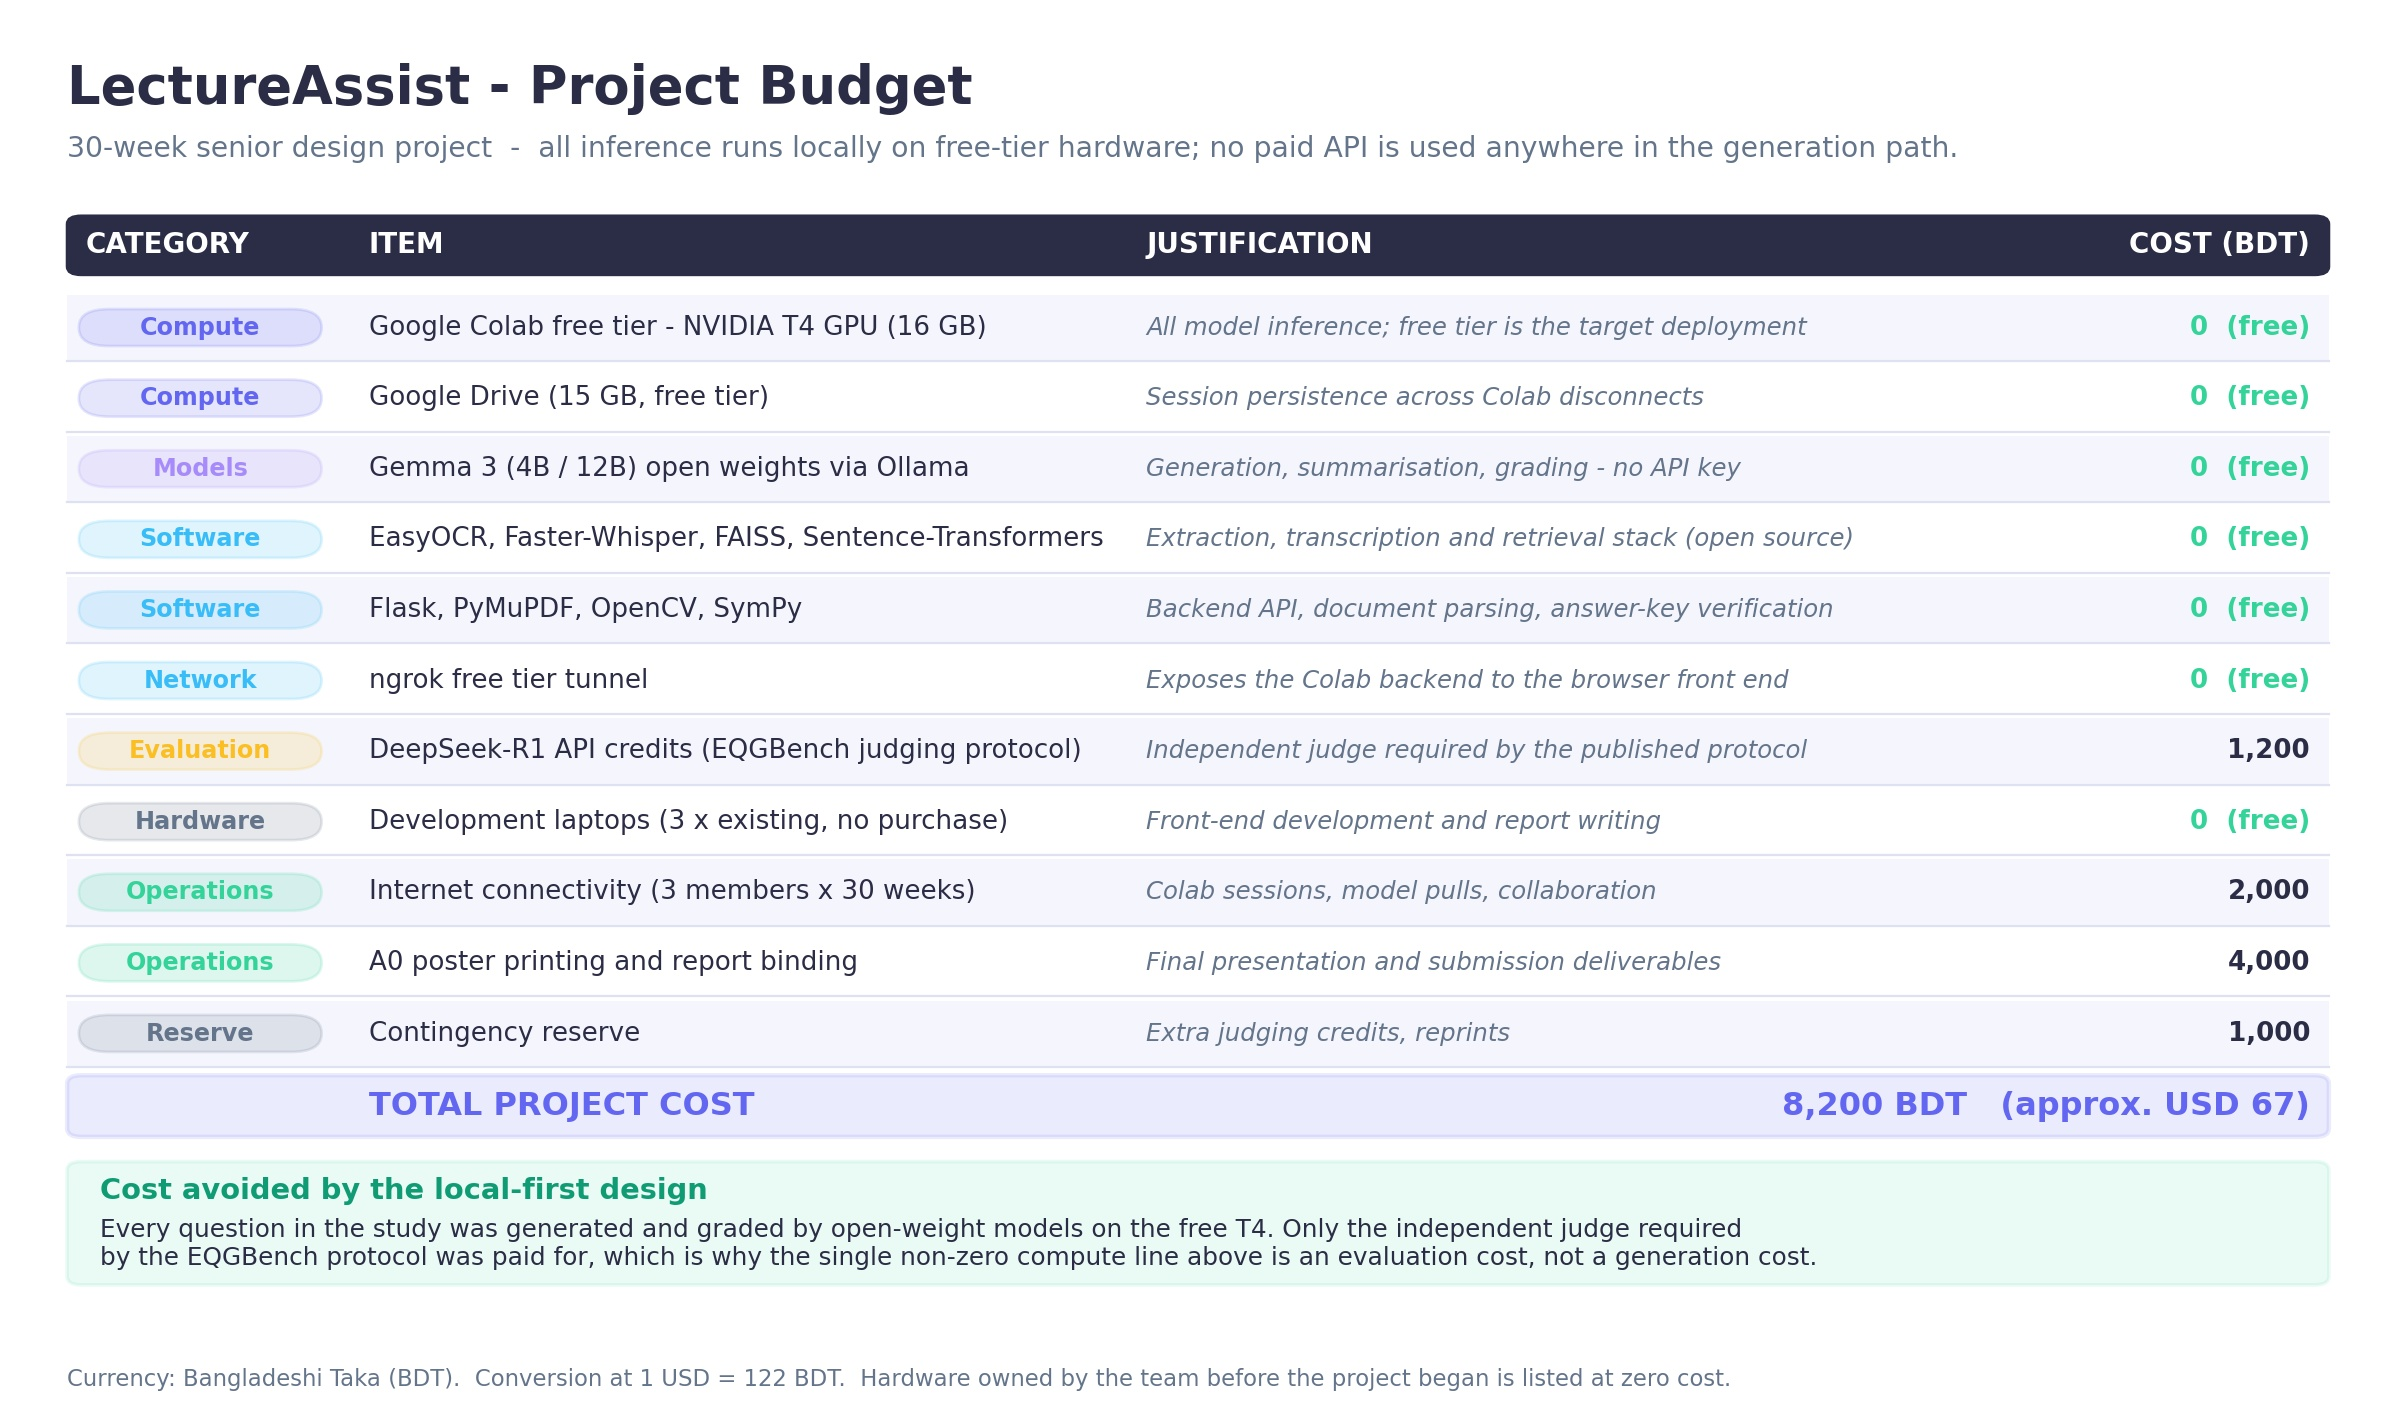
\includegraphics[width=\linewidth]{budget_table.jpg}
\caption{Project budget. Every component on the generation path is free: the compute
is a free-tier NVIDIA T4, the models are open weights served locally, and the
extraction, retrieval and serving stack is open source. The single non-zero technical
line is the independent judge required by the EQGBench protocol, which is an
evaluation cost rather than a system cost.}
\label{fig:budget}
\end{figure}

The structure of that table is the point of it, more than the total. Three
observations follow.

\paragraph{The system itself costs nothing to run.} Every line associated with
producing study material, compute, models, extraction stack, retrieval, serving,
is zero. This is a direct consequence of the constraint stated in
Chapter~\ref{ch:impacts}: a tool whose purpose is to make high-volume retrieval
practice available to students who cannot afford per-token cloud pricing cannot
itself depend on per-token cloud pricing. The engineering cost of that decision is
real and is paid elsewhere in this report: it is why the generator is a $4$B
model, and why so much of Chapter~\ref{ch:methodology} is concerned with extracting
reliable structured output from a small model.

\paragraph{The one paid line is a measurement cost, not a product cost.} EQGBench
specifies DeepSeek-R1 as its judge, and a faithful reproduction of a published
protocol requires using the model the protocol specifies. Substituting a locally
served model would have made the numbers incomparable with the published figures,
which is the entire reason for implementing the protocol faithfully in the first
place. A user of LectureAssist never incurs this cost; only a party reproducing the
evaluation does.

\paragraph{The dominant real cost is human time, which does not appear in the table.}
Roughly $2{,}000$~BDT of the total is connectivity and $4{,}000$~BDT is printing and
binding, so the budget is dominated by overheads that any project of this length
would incur regardless of its subject. The genuine investment in this project was the thirty weeks of work documented
in Section~\ref{sec:plan-gantt}, and the fact that a system of this scope could be
built and evaluated for well under USD~$100$ of direct cost is itself a result worth
recording, since it establishes that the approach is reproducible by any student team
with a laptop and an internet connection.

\paragraph{Cost avoided.} It is worth stating what the alternative would have been.
The evaluation reported in Chapter~\ref{ch:results} involved generating hundreds of
questions per pipeline configuration, each of which consumed multiple LLM calls under
the agentic loop, and then judging every resulting question. Executed against a
commercial frontier API at prevailing per-token rates, that workload would have cost
one to two orders of magnitude more than the entire budget above, and, critically,
it would have made the ablation and merging experiments of
Section~\ref{sec:res-ablation} unaffordable, since those multiply the corpus by the
number of configurations under test. Running locally did not merely save money; it
made a class of experiment possible that would otherwise have been out of reach.

\chapter{Complex Engineering Problems and Activities}
\label{ch:cep}

This chapter maps LectureAssist onto the Complex Engineering Problem (CEP) and
Complex Engineering Activity (CEA) attributes, showing where the project required
depth of knowledge, resolution of conflicting requirements, and analysis beyond the
routine application of a known method. Each attribute is addressed with reference to
the specific decision, defect or measurement in this report that exercises it, rather
than by general assertion.

\section{Complex Engineering Problems (CEP)}
\label{sec:cep}

{\footnotesize\singlespacing
\begin{longtable}{|c|p{3.4cm}|p{8.4cm}|}
\caption{Complex Engineering Problem attributes addressed by LectureAssist.}
\label{tab:cep}\\
\hline
\textbf{Attr.} & \textbf{Description} & \textbf{How the project addresses it} \\
\hline
\endfirsthead
\hline
\textbf{Attr.} & \textbf{Description} & \textbf{How the project addresses it} \\
\hline
\endhead
\hline
\endfoot
\hline
\endlastfoot

P1 & Depth of knowledge required (K3--K8) &
The system spans computer vision and image preprocessing for scene-adaptive OCR
(K3--K4), automatic speech recognition, transformer language models, embeddings and
vector retrieval (K4--K5), multi-agent software architecture and API/system design
(K5--K6), statistical evaluation design, LLM-as-judge, $F_1$ agreement between the
internal validator and an independent judge, calibration against a known-answer set
(K5, K8), and the research literature on question generation, chain-of-thought and
program-of-thought prompting, and agentic architectures (K8). \\
\hline
P2 & Range of conflicting requirements &
Several requirements pull directly against each other. \emph{Question quality vs.\
cost}: the agentic loop produces better-grounded, less repetitive and more
answer-correct questions but consumes roughly an order of magnitude more LLM calls
than a single-shot request. \emph{Model size vs.\ VRAM}: a larger generator would
produce better questions, but the generator, judge, Whisper, OCR and embedding models
must all coexist on one $16$\, GB T4. \emph{Yield vs.\ scientific honesty}: allowing
the $4$B generator to escalate to the $12$B model on malformed output would have
raised yield, but would have falsified the claim that the questions were written by
the $4$B, so escalation was disabled at a known cost in yield. \emph{Accept rate
vs.\ diversity}: a pipeline can maximise its accept rate by repeatedly producing one
good question, which forced the adoption of a duplicate-penalised effective
acceptance metric (Eq.~\ref{eq:effaccept}) in place of raw acceptance. \\
\hline
P3 & Depth of analysis required &
There is no unique correct design, and no off-the-shelf metric for ``is this a good
generated question''. Selecting a solution required analysing four generation
strategies (agentic, plain, CoT, PoT) against each other under a metric suite that
had itself to be designed, and it required identifying and eliminating confounds,
unequal content coverage between pipelines, a truncated summary that made whole
sections of the chapter unreachable by the planner, and silent model escalation,
any one of which would have invalidated the comparison. The central analytical
finding is that the four judged quality dimensions \emph{saturate} and therefore
discriminate nothing, so that the entire result rests on corpus-level automated
measures that a conventional quality-only evaluation would never have computed. That
conclusion is invisible without the analysis and inverts the naive reading of the
data. \\
\hline
P4 & Familiarity of issues &
The project integrates infrequently encountered components: EasyOCR with
scene-dependent preprocessing, Faster-Whisper, Gemma~3 served through Ollama,
Sentence-BERT embeddings, a FAISS index, an LLM-as-judge evaluation harness, SymPy
for machine-verified answer keys, and a Flask/ngrok deployment onto ephemeral
free-tier GPU infrastructure. \\
\hline
P5 & Extent of applicable codes &
No standard or code of practice exists for automatic educational question generation
or for the evaluation of LLM-generated assessment items. The evaluation protocol,
what to measure, how to verify an answer, how to calibrate the judge, had to be
designed from the research literature rather than taken from a standard. Where
published protocols did exist they had to be reconstructed from the papers
themselves: EQGBench has no public code release, and ReQUESTA publishes no judge
prompt at all because its rubric was applied by human raters. \\
\hline
P6 & Extent of stakeholder involvement &
Stakeholders include students (the primary users), instructors (whose lectures are
the input and whose assessments the tool must not undermine), institutions (which
hold copyright in lecture material and are accountable for academic integrity), and
the open-model community whose licences govern the deployed models. Their
requirements conflict: a student wants unlimited questions immediately, while an
instructor requires that the tool not present unverified answers as authoritative,
and an institution requires that copyrighted lecture material not be transmitted to a
third-party processor. \\
\hline
P7 & Interdependence &
The subsystems are tightly coupled: OCR and ASR quality bound the summary; the
summary bounds the planner's topic choice; the planner bounds question diversity; the
retrieval index bounds grounding; and the judge and Answer Generator bound the
credibility of every reported result. Two of the defects found during this project, a truncated summary and a capped content window, were failures of exactly this
interdependence: a bug several stages upstream degraded question diversity many
stages downstream, with no local symptom at the point of failure. The pipeline
labelling error disclosed in Section~\ref{sec:res-native} is a third instance, in
which a fault in the recording of provenance propagated into the interpretation of
every downstream measurement. \\
\hline
\end{longtable}
}

Table~\ref{tab:cep} shows that the project engages all seven CEP attributes, with P2
(conflicting requirements) and P3 (depth of analysis) being the most heavily
exercised. It is worth noting that P2 and P3 are linked in this project rather than
independent: almost every conflicting requirement listed under P2 was resolved by
\emph{measuring} the trade-off rather than by asserting a preference, and the
instruments built to perform those measurements are what generated the depth of
analysis recorded under P3.

\section{Complex Engineering Activities (CEA)}
\label{sec:cea}

{\footnotesize\singlespacing
\begin{longtable}{|c|p{3.4cm}|p{8.4cm}|}
\caption{Complex Engineering Activity attributes addressed by LectureAssist.}
\label{tab:cea}\\
\hline
\textbf{Attr.} & \textbf{Description} & \textbf{How the project addresses it} \\
\hline
\endfirsthead
\hline
\textbf{Attr.} & \textbf{Description} & \textbf{How the project addresses it} \\
\hline
\endhead
\hline
\endfoot
\hline
\endlastfoot

A1 & Range of resources &
The project draws on human resources (a three-member team with a supervisor), modern
computational tools (a GPU runtime, six distinct deep-learning models, a vector
index, a symbolic algebra system), open-licensed source material, and cloud compute, managed under a hard constraint of zero paid API spend on the generation path,
as documented in the budget of Section~\ref{sec:plan-budget}. \\
\hline
A2 & Level of interactions &
The work required interaction between the extraction, retrieval, generation,
evaluation and interface subsystems, each with its own failure modes, as well as
between team members under the responsibility allocation of
Table~\ref{tab:raci}, the project supervisor (whose requirements shaped the
evaluation design, notably the demands for CoT and PoT baselines and for treating
question generation and answer generation as separate cross-checked agents), and the
end users whose trust in the output determines whether the system is safe to use. \\
\hline
A3 & Innovation &
The project introduces three novel elements: scene-adaptive OCR that classifies each
frame before choosing its preprocessing, so that a lecture's \emph{board}: not
merely its audio, becomes usable content; a validator agent that selects
\emph{how} to remediate a rejected question (regenerate, fetch more context, or
replan the topic) rather than merely rejecting it; and an evaluation protocol that
separates question quality from answer correctness by having a distinct Answer
Generator agent re-solve every question blind, with the solver itself calibrated on a
machine-verified answer key. \\
\hline
A4 & Consequences to society and the environment &
The system widens access to effective retrieval practice for students who cannot pay
for cloud AI services, supporting UN SDG~4 (Quality Education) and SDG~10 (Reduced
Inequalities). Running small models locally is substantially less energy-intensive
per request than hyperscale cloud inference, and no model was trained. The principal
risk, a fluent question with a wrong marked answer, is analysed and bounded
rather than dismissed, and the report states explicitly that generated questions are
suitable for practice and not for graded assessment without human review.
Chapter~\ref{ch:impacts} develops these consequences in full. \\
\hline
A5 & Familiarity &
The project requires familiarity with computer vision, speech recognition, large
language models and prompting strategies, retrieval-augmented generation, agentic
architectures, experimental design and statistical evaluation, web API development,
and deployment onto constrained, ephemeral GPU infrastructure. \\
\hline
\end{longtable}
}

Table~\ref{tab:cea} demonstrates that the project satisfies all five Complex
Engineering Activity attributes.

\section{Mapping to Knowledge Profiles}
\label{sec:cep-knowledge}

Table~\ref{tab:knowledge} records which Washington Accord knowledge profiles the work
draws on and where in this report the evidence for each can be found, so that the
mapping can be checked against the substance of the project rather than accepted on
assertion.

{\footnotesize\singlespacing
\begin{longtable}{|c|p{5.0cm}|p{6.4cm}|}
\caption{Knowledge profile coverage and where each is evidenced in this report.}
\label{tab:knowledge}\\
\hline
\textbf{Profile} & \textbf{Description} & \textbf{Evidence in this report} \\
\hline
\endfirsthead
\hline
\textbf{Profile} & \textbf{Description} & \textbf{Evidence in this report} \\
\hline
\endhead
\hline
\endfoot
\hline
\endlastfoot

K3 & Engineering fundamentals &
Image preprocessing, contrast-limited adaptive histogram equalisation,
thresholding, polarity inversion, selected per frame class
(Section~\ref{sec:meth-ocr}) \\
\hline
K4 & Engineering specialist knowledge &
Transformer language models, speech recognition, sentence embeddings and
approximate nearest-neighbour search (Chapter~\ref{ch:background}) \\
\hline
K5 & Engineering design &
The five-agent Plan--Retrieve--Generate--Validate--Refine architecture and its
alternatives (Section~\ref{sec:meth-agentic}, Figure~\ref{fig:agentic-loop}) \\
\hline
K6 & Engineering practice &
Component selection against stated alternatives and rationale
(Table~\ref{tab:tools}); deployment on constrained infrastructure \\
\hline
K7 & Comprehension of the role of engineering in society &
Access, safety, privacy and environmental analysis (Chapter~\ref{ch:impacts}) \\
\hline
K8 & Research literature &
Two published protocols reconstructed from their source papers and applied with
declared deviations (Section~\ref{sec:res-protocol}) \\
\hline
\end{longtable}
}

\chapter{Conclusion}
\label{ch:conclusion}

This chapter summarises what was built and what was learned, states the limitations
of the work honestly, and sets out the improvements that follow most directly from
them.

\section{Summary}
\label{sec:concl-summary}

LectureAssist is an end-to-end, fully local agentic system that turns a raw lecture
video or academic document into validated, difficulty-controlled study and assessment
material. It fuses two extraction channels --- scene-adaptive OCR that classifies each
frame before preprocessing it, so that slides, blackboards, whiteboards and on-screen
text are each handled correctly, and Faster-Whisper speech transcription --- into a
single timestamped lecture timeline. That timeline is summarised, chunked, embedded
and indexed, and then consumed by a multi-agent pipeline that plans questions across
topics, retrieves its own evidence when it judges its context insufficient, generates
one question at a time, validates each against difficulty, grounding and instruction
compliance, and, on failure, chooses \emph{how} to remediate before retrying. Around
this sit a retrieval-grounded chat interface, a multi-tier grader that falls back from
exact matching through fuzzy similarity to LLM rubric evaluation, and an adaptive
engine that steers subsequent quizzes toward the topics a student is weakest on.
Everything runs on open-weight Gemma~3 models served locally through Ollama on a
single free-tier GPU, with no paid API anywhere in the system.

The project's second contribution is an evaluation that takes seriously a question the
field usually does not ask: not \emph{does the generator write good questions}, but
\emph{does it mark the right answer}. Question generation and answer generation are
treated as two distinct agents, and their answers are cross-checked by having a
larger model re-solve every question without seeing the marked option. Measured this
way against a plain single-shot baseline on a college calculus chapter, the agentic
pipeline wins on judged quality at every difficulty and wins decisively on answer
correctness where it matters most --- $99\%$ versus $81\%$ judge-verified on hard
questions --- at roughly seven times the wall-clock cost.

The most instructive result, however, is a negative one. Judge scores turned out to be
compressed near the ceiling and to discriminate poorly between pipelines, while the
duplicate rate discriminated sharply; and at hard difficulty the agentic pipeline
collapses onto a narrow slice of the chapter and repeats itself so badly that a
repetition-aware metric ranks the plain baseline \emph{above} it. A quality-only
evaluation --- the kind most commonly reported --- would have shown the agentic
pipeline winning cleanly across the board and would have concealed this entirely.

\section{Limitations}
\label{sec:concl-limits}

\paragraph{The judge and the Answer Generator are LLMs, not humans.} All quality
scores are produced by \texttt{gemma3:12b} rather than by human raters. LLM judges are
known to reward fluency and verbosity, and the judge here shares a model family with
the generator, so it plausibly shares its blind spots. Absolute scores should be read
as a relative signal between pipelines, not as an objective measure of question
quality.

\paragraph{The Answer Generator is weak, which bounds every answer-correctness
number.} On the known-answer calibration set the solver scores only $55\%$, and the
generator model $70\%$. Generator--solver agreement of $88$--$97\%$ therefore cannot be
interpreted as that fraction of questions being verifiably correct; two models from
the same family agree partly because they behave alike. This is why the calibration is
reported --- but it means the answer-correctness results establish a ranking between
pipelines, not a trustworthy absolute correctness rate. A stronger or
non-Gemma solver would tighten this considerably.

\paragraph{The CoT and PoT comparison is not yet complete.} The four-pipeline run is
implemented and the prompts are fixed, but the completed measurements reported in
Chapter~\ref{ch:results} cover the agentic versus plain non-agentic comparison; the
CoT and PoT rows are shown as pending rather than filled with estimates.

\paragraph{Single domain, single document.} All results come from one chapter of one
subject (limits, from OpenStax \emph{Calculus, Volume~1}). Mathematics is unusually
favourable to program-of-thought prompting and unusually hostile to OCR, and nothing
here establishes that the findings transfer to a humanities lecture or to a
lab-based science course.

\paragraph{The extraction layer bounds everything above it.} OCR on handwritten
board work is imperfect, transcription degrades with accent and background noise, and
mathematics rendered as an image in a PDF is not extracted at all. Every defect in
extraction propagates silently upward: a missing board block looks exactly like a
board that was never written on, and the question generator has no way to know that
material is absent.

\paragraph{The agentic pipeline's diversity failure at hard difficulty is unresolved.}
It is measured, diagnosed --- the planner and retriever converge on the narrow region
of the chapter that supports difficult questions, and each retry draws from that same
region again --- and reported, but not yet fixed.

\paragraph{Deployment is not production-grade.} The system runs on a free Colab
runtime behind an ngrok tunnel, with a single-user interface, no authentication, and
session state on Google Drive. This is adequate to demonstrate and evaluate the
system; it is not a deployable service.

\section{Future Improvement}
\label{sec:concl-future}

\paragraph{Fix the diversity collapse first.} It is the clearest defect the evaluation
exposed and the one that currently negates the agentic pipeline's advantage on hard
questions. Two mechanisms follow directly from the diagnosis: maintain a coverage map
of which regions of the document have already been used and penalise the planner for
returning to them, and make the generator aware of the questions already produced in
the current run so that a retry is required to be \emph{different}, not merely
\emph{valid}. A duplicate check could also be moved inside the validation loop, so
that a repetitive question is rejected at generation time rather than discovered at
evaluation time.

\paragraph{Strengthen answer verification.} The weakest link in the evaluation is the
solver. Verifying computational answers symbolically with SymPy --- as is already done
when constructing the calibration set --- would replace an LLM's opinion with a
machine-checked fact for exactly the question type where the generator is most likely
to be wrong. Using a solver from a different model family, or an ensemble, would
break the shared-blind-spot problem that currently inflates the agreement rate.

\paragraph{Human evaluation.} A modest human study --- a few instructors rating a
sample of generated questions, and independently answering them --- would anchor the
LLM judge to a ground truth and quantify how far its scores can be trusted. This is
the single highest-value addition to the evaluation.

\paragraph{Broaden the domain.} Repeating the comparison on a non-mathematical subject
would test whether the agentic advantage in answer correctness is general or is an
artifact of a domain in which answers are computed and therefore easy to get wrong.

\paragraph{Complete and extend the pipeline comparison.} Finishing the CoT and PoT
runs will answer whether a better prompt can recover most of the agentic pipeline's
benefit at a fraction of its cost --- a question with direct practical consequences,
given the seven-fold cost difference. A hybrid worth testing is a CoT or PoT generator
placed \emph{inside} the agentic validate-and-retry loop, combining derived answers
with external validation.

\paragraph{Productionisation.} Multi-user support with authentication, a persistent
server rather than an ephemeral notebook runtime, and quantised models for lower-VRAM
consumer GPUs would move the system from a demonstrated prototype toward something a
class of students could actually use.




\addcontentsline{toc}{chapter}{References}

\clearpage
%\appendix 

%\phantomsection

%\addcontentsline{toc}{chapter}{Appendices}
%\chapter{Amino Acids\label{appAmino}}
%\begin{figure}[h]
%\begin{center}
%\includegraphics[width=1\textwidth]{./images/background/aminoacids}
%\end{center}
%\caption{Twenty different amino acids, their structures and chemical properties.\index{Amino Acid!chemical properties}\cite{Lehninger2012}.}
%\end{figure}
%\clearpage
%\thispagestyle{empty}
%\mbox{}

%\clearpage
%\phantomsection
%\addcontentsline{toc}{chapter}{Index}
%\printindex
\bibliographystyle{IEEEtran}
\bibliography{references}
\end{document}
